\documentclass[letterpaper, 12pt]{article}
\title{Gnuspeech ``Monet''}
\usepackage{wrapfig}
\usepackage{lipsum}
\usepackage{media9}
\usepackage{graphicx}
\usepackage{geometry}
\usepackage{hyperref}
\usepackage{amsmath}
\usepackage{amssymb}
\usepackage{MnSymbol}
\usepackage{afterpage}
\usepackage[justification=centering]{caption}
\usepackage{xcolor}
\usepackage{natbib}

\def\bsq#1{%both single quotes
\lq{#1}\rq}

\newlength{\myMheight}
\settoheight{\myMheight}{12pt}
\usepackage{tipa}
\newcommand{\ipauh}{\textschwa}
\newcommand{\ipaa}{\textturnv}
\newcommand{\ipae}{\textepsilon}
\newcommand{\ipai}{\textiota}
\newcommand{\ipao}{\textopeno}
\newcommand{\ipau}{\textcloseomega}
\newcommand{\ipaaa}{\ae}
\newcommand{\ipaee}{i}
\newcommand{\ipaer}{\textschwa :}
\newcommand{\ipaar}{\textscripta}
\newcommand{\ipaaw}{\textopeno :}
\newcommand{\ipaei}{\textepsilon\textiota}
\newcommand{\ipauhuu}{\textturnv\textcloseomega}
\newcommand{\ipaahuu}{\ae\textcloseomega}
\newcommand{\ipaoi}{o\textiota}
\newcommand{\ipaahi}{\ae\textiota}
\newcommand{\ipaw}{w}
\newcommand{\ipay}{j}
\newcommand{\ipar}{r}
\newcommand{\ipal}{l}
\newcommand{\ipap}{p}
\newcommand{\ipat}{t}
\newcommand{\ipak}{k}
\newcommand{\ipab}{b}
\newcommand{\ipad}{d}
\newcommand{\ipag}{g}
\newcommand{\ipam}{m}
\newcommand{\ipan}{n}
\newcommand{\ipang}{\textipa{N}}
\newcommand{\ipas}{s}
\newcommand{\ipaf}{f}
\newcommand{\ipath}{\textipa{T}}
\newcommand{\ipash}{\textesh}
\newcommand{\ipaz}{z}
\newcommand{\ipazh}{\textipa{Z}}
\newcommand{\ipav}{v}
\newcommand{\ipadh}{\textipa{D}}
\newcommand{\ipach}{\textteshlig}
\newcommand{\ipaj}{\textdyoghlig}
\newcommand{\ipah}{h}

\newcommand{\wbstuh}{\textschwa}
\newcommand{\wbsta}{\textprimstress\textschwa}
\newcommand{\wbste}{e}
\newcommand{\wbsti}{i}
\newcommand{\wbsto}{\textipa{\"a}}
\newcommand{\wbstu}{\.u}
\newcommand{\wbstaa}{a}
\newcommand{\wbstee}{\=e}
\newcommand{\wbster}{\oe}
\newcommand{\wbstar}{\.a}
\newcommand{\wbstaw}{\.o}
\newcommand{\wbstei}{\=a}
\newcommand{\wbstuhuu}{\=o}
\newcommand{\wbstahuu}{a\.u}
\newcommand{\wbstoi}{\.oi}
\newcommand{\wbstahi}{\=\i}
\newcommand{\wbstw}{w}
\newcommand{\wbsty}{y}
\newcommand{\wbstr}{r}
\newcommand{\wbstl}{l}
\newcommand{\wbstp}{p}
\newcommand{\wbstt}{t}
\newcommand{\wbstk}{k}
\newcommand{\wbstb}{b}
\newcommand{\wbstd}{d}
\newcommand{\wbstg}{g}
\newcommand{\wbstm}{m}
\newcommand{\wbstn}{n}
\newcommand{\wbstng}{\textipa{N}}
\newcommand{\wbsts}{s}
\newcommand{\wbstsh}{sh}
\newcommand{\wbstf}{f}
\newcommand{\wbstth}{th}
\newcommand{\wbstz}{z}
\newcommand{\wbstzh}{zh}
\newcommand{\wbstv}{v}
\newcommand{\wbstdh}{\underline{th}}
\newcommand{\wbstch}{ch}
\newcommand{\wbstj}{j}
\newcommand{\wbsth}{h}



\geometry{letterpaper,textwidth=16cm,textheight=24.5cm}

% End of preamble
%The body now follows

\begin{document}
\pagenumbering{roman}

\setlength{\topmargin}{-2.5cm}
\vspace*{4cm}
\begin{flushleft} {\LARGE \textbf{Gnuspeech Monet Manual 0.9}}\end{flushleft}
\noindent
\rule[6mm]{16cm}{1.5mm}
\vspace{-1.3cm}
\noindent
\begin{flushright} {\small{Gnuspeech: the speech synthesis database creation, \\modification, and articulatory synthesis software suite}}\end{flushright}



\vspace{12cm}

\begin{flushleft} {\Large \textbf{David R. Hill, University of Calgary}}\end{flushleft}
\rule[7mm]{16cm}{0.9mm}
\vspace{-1.3cm}
\begin{flushleft} {\small{Based on work over more than three decades by the author, Leonard Manzara, Craig Schock, Ian Witten, Wiktor Jassem, Steve Nygard, Dalmazio Brisinda, Marcelo Matuda, and many talented undergraduate students (See \href{http://www.gnu.org/software/gnuspeech}{``Thanks to those who have helped'' http://www.gnu.org/software/gnuspeech}, accessed 2015-07-24). Thanks also to Richard Stallman and the Gnuisances, Karl Berry and Brandon Invergo at the Free Software Foundation for their enlightened support.}}\end{flushleft}

\newpage

\vspace*{8 cm}
\noindent{}Copyright \textcopyright{} 2002, 20012, 2015  David R. Hill

\vspace{12 pt}

\noindent{}This manual is for Gnuspeech version 0.9, 23 August  2015

\vspace{12 pt}

\noindent{}Permission is granted to copy, distribute and/or modify this document under the terms of the GNU Free Documentation License, Version 1.3 or any later version published by the Free Software Foundation; with no Invariant Sections, no Front-Cover Texts, and no Back-Cover Texts.

\vspace{12 pt}

\noindent{}A copy of the license is available at: \href{http://www.gnu.org/licenses/fdl-1.3.en.html} {http://www.gnu.org/licenses/fdl-1.3.en.html---the Free Software Foundation site (accessed 2015-08-15)}

\newpage

\section*{Summary}
{Monet}\footnote{``\underline{M}y \underline{O}wn \underline{N}ifty \underline{E}diting \underline{T}ool'', designed and implemented by Craig Schock as the system architect for the original NeXT computer version, to provide the foundation tool for creating ``event-based'' speech data based on earlier and ongoing research by the author. Both the creation of the system, and its use to develop the articulatory speech databases, involved sufficient artistry that it seems very appropriate to maintain the artistic name connection. The current system is mostly ported to both GNU/Linux and the Macintosh. The implementation of Gnuspeech under GNUStep is reasonably well documented by the original NeXT manual that also accompanies this release, though it needs to be updated (real soon now!).} comprises three main divisions serving distinct functions: (1) a Speech Server that translates ordinary text into spoken output, via a specialised phonetic script with automatically added rhythm and intonation information; (2) a speech synthesis database editor and manager with a Graphical User Interface (GUI); and (3) a GUI front end to the Speech Server that is intended to allow databases to be tested as they are developed, but also allows the speech synthesis to be evaluated, including the effects of intonation, and can provide carefully managed test utterances for subjective testing.

These divisions form the core of the Gnuspeech software, providing: (1) real-time articulatory speech synthesis; and (2) providing databases creation facilities for arbitrary languages, research facilities for linguistics research, speech therapy, language-learning, and other speech-research-related topics. A platform-independent synthesis engine---GnuspeechSA---provides command-line access to the speech synthesis capability (See Appendix \ref{matuda}).

Monet was one of two primary tools used to create the original databases for the spoken English that can now be produced. The other tool was an interactive application, currently known as \textit{TRAcT}\footnote{ TRAcT---\underline{T}ube \underline{R}esonance \underline{Ac}cess \underline{T}ool---is available as part of this GNU project release, and includes a manual. TRAcT allows a user to experiment with static configurations of the vocal tract model that provides the low-level articulatory-synthesis waveform-output from the system (and from standalone use of the Speech Server), and was necessary in developing the configurations, or ``postures'' whose dynamic variation produce speech.} Two other important helper tools are also involved in the process of creating new databases: a basic editor to compile the pronouncing dictionary that is used (Monet has a dictionary of over 70,000 words, plus a means of constructing derivatives); and a means of generating detailed sound spectrograms of utterances to validate the correctness of both static and dynamic sounds being developed using Monet. In connection with the dictionary, a letter-to-sound converter is highly desirable to catch any words that cannot be found or constructed using the dictionary.

The original complete ``TextToSpeech'' kits that represented the NeXT Computer implementation also included auxiliary applets, most notably ``BigMouth'' that used the Speech Server to speak files, speak scratch-pad text, and vary some speaker characteristics, and ``PrEditor'', that can be used to create dictionaries specific to a particular user, or a particular application. These are not yet ported and will be the subject of later releases. The functions associated with database creation are not completely ported, but are described as if complete to guide those who continue to work on the port and further development.

This manual provides a description of the structure and use of Monet together with selected tables of the data used by the system. A quick introduction to GnuspeechSA on the Macintosh is also provided.

\newpage
\vspace{12cm}
[This page is intentionally blank]
\newpage
\tableofcontents
\newpage
\pagenumbering{arabic}

\section{Purpose of the system }
Monet is a special purpose interactive GUI-based editing system built to facilitate the creation and modification of databases that allow computer synthesis of spoken language. Monet has a recursive flavour---in order to carry out its function it must include a means of speaking the rudiments language it is developing, achieved by ensuring ``speech'' can be produced even before \textit{any} data, apart from one posture, has been entered.

\section{System capabilities}
The current version of Monet, shown in Figure \ref{mon-ov} includes:
\begin{enumerate}
\item{The real-time ``Speech Server''\footnote{the Speech Server is also the core of the cross-platform applications related to speech output developed by Marcelo Matuda that are part of this release. (See Appendix \ref{matuda}} that converts text to phonetic descriptions, to synthesiser parameters, and thence into a speech waveform. The Speech Server comprises:}
\begin{enumerate}
\item{a database containing posture data (including, but not limited to: tube radii; marked and unmarked durations; rules for combining \emph{n}-phones; transition shapes used by the rules; and special transitions for things like noise-bursts and micro-intonation);}
\item{a parsing module for pre-processing ordinary text to account for the conventions specific to the target language (such as how dates and acronyms should be pronounced);}
\item{a pronouncing dictionary with methods for creating derived words;}
\item{a language-specific set of letter-to-sound rules to convert words for which there is no dictionary entry or derived word;}
\item{a waveguide (``tube'') model of the human vocal apparatus to perform the conversion of parameters into a speech waveform for output;}
\item{a computational model of rhythm, applied to the phonetics, based on natural speech data derived from the specific target language---English in this case;} and
\item{a computational model of intonation---the rise and fall of pitch---based on language-specific linguistic models available in the literature and refined/tested by subjective experiment. Such a model is actually not practical in early development of a language database and we used monotone in the English development and added the intonation module later, though some simple pitch movement allowed a better assessment of results.}
\end{enumerate}

\item{GUI-based access to the Speech Server, with informative displays and controls:}
\begin{enumerate}
\item{a ``Synthesis Window'' that allows entry of text or posture strings that are to be spoken, as well as allowing the thirty-two articulatory control parameters (sixteen regular and sixteen special) to be plotted and displayed, along with timing and posture-type information. The speech events can be displayed, the graph images saved, and the input synthesised to provide speech output, or sent to a sound file. It uses the Speech Server for synthesis and is essential for checking the developing database when developing a new one, or modifying an existing one, as well as allowing the creation of stimuli for subjective testing;}
\item{a ``Synthesizer Control Panel'' that allows the ``Control Rate'' parameters (such as vocal tract--tube--length, and nasal passage radii) to be set;} 
\item{an ``Intonation Window'' that provides a graph of the intonation contour, showing the postures and timing. It includes the ability to modify the contour;}
\item{an ``Intonation Settings'' window providing control of the intonation contour parameters (such as component ranges, and whether smoothing is applied) and allows the speech ``Tempo'' to be changed.}
\end{enumerate}

\item{A special-purposes GUI-based editor---not yet fully ported---that provides the ability to create and edit the databases used by the Speech Server. It includes:}
\begin{enumerate}
\item{entry of posture names, parameter values, timing, and categories;}
\item{means for creating prototypes for parameter transitions, based on arbitrary timing points with chosen descriptive names. The transitions are not shapes \textit{per se}, but are graphs showing the percentage change from one target to the next, plotted against time, and showing the designated timing points. Two kinds of transition prototypes are provided, regular and special. A Prototype Manager provides a higher-level means of managing these;}
\item{a rule manager that specifies which transition profiles should be applied to which combinations of postures for which parameters. If postures are thought of as phones, provision is made for \textit{n}-phone combinations, where \textit{n} varies from 2 to 4 (an isolated phone still requires transitions from and to silence);}
\item{a rule tester to make it possible to see which rules will apply to a given string of postures as they are entered into the tester and shifted.}
\end{enumerate}
\end{enumerate}


\begin{figure}[htb]
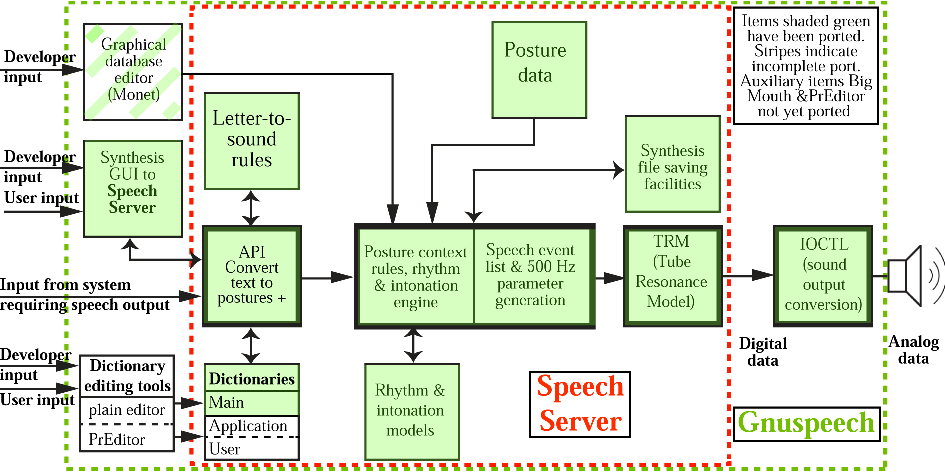
\includegraphics{./images/Gnuspeech-block-diagram-greened-revised-16-new}
\caption[Overview of Monet]{\label{mon-ov}Overview of Monet, showing components ported so far}
\end{figure}

The TRAcT manual that is part of this release provides background on the origins of speech synthesis and the progress that has been made, as well as the technical details of the waveguide vocal tract model or ``Tube Resonance Model'' (TRM). The TRM is properly thought of as a low-level synthesiser as opposed to the complete system which is a high-level synthesiser. The low level synthesiser is akin to a trumpet---it only plays music when operated by a trained trumpet player (the player is analogous to the high-level control that produces speech from the low-level synthesiser). Papers describing the original research used to establish  the databases, the rhythm model, and the intonation model, are cited.The most recent paper (Hill 2015) gives more detail on the background, and outlines the procedure by which the databases were created. The work is all original, drawing on long-term research in many laboratories, other university departments, and by team members in the author's laboratory, as well as members of the Trillium Sound Research team. Trillium Sound Research was a University of Calgary technology spin-off company that created the original NeXT implementation of the system (then known as various levels of the ``TextToSpeech Kit''). The company was dissolved, and the software donated to the Free Software Foundation (FSF) under a General Public Licence and General Document Licence---hence the GNU Project ``Gnuspeech''. Acknowledgements appear, amongst other places, on the \href{http://www.gnu.org/software/gnuspeech}{http://www.gnu.org/software/gnuspeech---Gnuspeech home page which is on the FSF site} ( accessed 2015-06-05).

\section{Introduction}
Unrestricted speech synthesis-by-rules efforts have often used methods developed
in the 50s and 60s to simulate speech production by feeding information about spectral features to a source-filter model of the vocal apparatus. The devices comprise a pulsed energy source, and a set of bandpass filters that imitate some of the excitation and resonant properties of the oral and sometimes nasal passages in the human head [e.g. Lawrence (1953); Fant (1956)]---``low-level synthesis''. As noted, ``high-level synthesis'' is then needed to provide the data and algorithms required to make the low-level synthesiser speak a particular language. Early work by other researchers provided the data and methods (high-level synthesis) needed to drive these models to produce synthetic speech---for example Liberman, \emph{et al.} (1959); Holmes \emph{et al.} (1964). The overall approach has been given a variety of names, but ``formant synthesis'' seems the most descriptive, since the variable driving data mainly comprise the centre frequencies of the resonances of the vocal tract\footnote{ The resonances correlate with the frequency peaks or ``formants'' in the output spectrum.} interacting with the energy input from the vocal folds, plus the various noises produced as a result of the passage of air through constrictions in the tract, including the vocal folds. ``DECtalk''---derived from Allen's (1987) ``MITalk''---is a formant synthesis approach. Formant synthesis is widely used---for example, by the distinguished physicist Stephen Hawking to allow him to ``speak'' despite his ALS, which prevents him from speaking naturally. Other systems are closely related. More recently ``concatenative synthesis'' has become popular. In this approach real speech is captured by some suitably sophisticated method (typically as Linear Predictive Coding---LPC, which allows easy separation of source excitation from the filtering effect of the vocal tract). The speech is segmented to collect suitable basic elements, and these are then rearranged and concatenated to produce new utterances. Although the speech is recognisably natural in sound quality, it suffers from: limitations inherent in the process which reduce the intelligibility: lack of natural intonation and rhythm; and difficulty in producing voices that have their own character distinct from the original recordings. Thus both formant and concatenation methods still suffer from restrictions of various kinds that interfere with the potential for naturalness in unrestricted speech---though, for restricted purposes, concatenated natural speech can be very effective. Waveform concatentation is the principle method underlying the Festival system at Edinburgh University's Centre for Speech Technology Research (CSTR undated). This project modularises the synthesis process so that researchers can work on a single module (say intonation management) without having to create and manage the entire synthesis process.

Mark Tatham's (2000) SPRUCE project at the University of Essex (UK) has been described as a system that provides the high level synthesis needed to drive both formant synthesis and concatenative synthesis. The emphasis appears to be on concatenative synthesis.

In 1993/4, building on fundamental work by Carr\'e, Fant and others (e.g. Fant \& Pauli 1974; Carr\'e \& Mrayati 1994), Cook (1989, 1991), Smith (1987a, 1987b) the author's team developed a speech synthesis system that uses a wave-guide approximation to the real vocal tract oral/nasal filter as the filter component, as opposed to individual filters for each formant, thereby providing an articulatory model---also called a ``tube model'', ``tube resonance model'' (TRM),  or ``waveguide model'' ( Hill \emph{et al.} (1995),). The work on the waveguide model at the Center for Computer Research in Music and Acoustics Stanford, by Julius Smith, Perry Cook and their colleagues, was a crucial element in the original NeXT implementation of their waveguide model, and the basic design has carried through into the current system. Such a model emulates\footnote{Emulate: to equal or surpass, especially by imitation} rather than simulates the resonant behaviour of the vocal tract because the tube model behaviour maps directly onto the articulatory and acoustic characteristics of the real vocal tract and nasal passage tube structures, rather than simply reproducing a partial output spectrum by some technical contrivance. For example, higher formants are produced naturally, and they vary, rather than having to be simulated by some form of fixed lumped-filter approximation. Also the nasal-oral energy balance is implemented directly, oral and nasal radiation are modelled directly, and so on.

\begin{wrapfigure}{L}{0.5\textwidth}
\centering
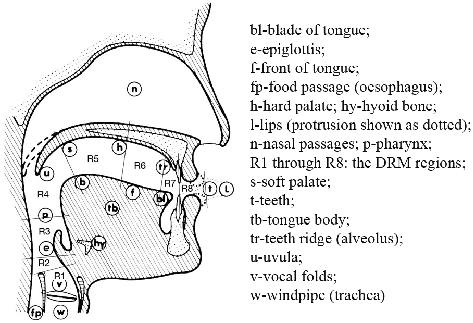
\includegraphics[width=0.45\textwidth]{images/sagittal-section-vocal-tract-r-drm}
\caption[DRM regions]{\label{main-men}DRM regions 1 through 8 shown nominally on a sagittal section of the head}
\end{wrapfigure}

The previous barriers to using a tube model for speech were three-fold. First there was the problem of controlling the many sections---typically 40---required for the tube approximation, in real-time, without instability or self-defeating approximations; secondly there was the problem of providing the complete database that represented the behaviour of many parts of a real vocal apparatus\footnote{Lungs, trachea, vocal folds, oral tube, tongue, teeth, cheeks, velum, nasal tube, lips, mouth orifice, and nostrils.} speaking a particular language; and thirdly, until the digital age, there was a problem with the stability of the analogue circuits that implemented the model. The work of Fant, Carr\'e and their colleagues (op. cit.) provided the theoretical basis for solving the control problem for the tube model. Based on a formant sensitivity analysis research by Fant and his colleagues, Carr\'e and Mrayati devised what they call the Distinctive Region Model (DRM) that provides a reasonably accurate model of articulation, that is related to the known properties of the real vocal tract, but requires only eight independently controlled sections instead of the forty or so that would be needed if the constraints of the vocal tract of speech were ignored. The topic is discussed more fully in the paper by Hill, Manzara \& Schock (1995) and in the manual for TRAcT that is part of this release. TRAcT is concerned with the TRM and its manipulation. The DRM control sections applied to the TRM correspond closely to the distribution of articulatory possibilities in the real vocal tract so that, even though the traditional parameters such as jaw rotation, tongue height, lip opening, and so on are not used directly, the model is truly an articulatory model, and the traditional parameters could be used at a meta-level to define the changes in the DRM regions. Provision for this intended extension has been made in the basic framework of the system.

A description of how the English database was built, what it contains, and why it has the form it has, appears in Hill (submitted).

In addition to the articulatory parameters that model the changes in the vocal apparatus associated with the succession of speech sounds Monet also models British English pitch contours to control the variation in pitch (intonation) over an utterance, as well as a rhythm model, based on extensive research in the author's university laboratory dealing with relative and absolute time duration of postures. It is the variation in posture durations that determines the rhythmic details of the speech that---in conjunction with the intonation---are so essential for excellent intelligibility. The rhythm model is explained in Hill, Jassem \& Witten (1979) and Jassem, Hill \& Witten (1984). The intonation model is broadly based on Halliday's model of intonation in spoken English (Halliday 1970), and is integrated with the rhythm model, as it must be. Indeed, it is not possible to describe the Halliday intonation model without also specifying a well-defined rhythmic structure.

In dealing with the machine perception and production of speech, a number of technical terms must inevitably be used in order to achieve precision of expression. The reader's attention is drawn particularly to the terms associated with speech sounds (phones, phonemes, postures, etc) and the basic concepts associated with rhythm and intonation. A ``conceptionary'' for speech and hearing in the context of machines and experimentation (Hill 1991) provides a convenient source of such conceptual knowledge.

Especially note that ``phonemes'' are \emph{not} speech sounds. They are \textit{categories} of speech sounds. Sounds fall in the same phoneme category for a given language if the difference between them does not distinguish between any two words in that language. Thus the sounds in a given phoneme category---called ``allophones''---may be quite varied acoustically, and may result from a variety of quite different articulatory causes. Sounds in the same phoneme category may be as different \emph{acoustically} as upper and lower case letters are different \emph{visually}. Consider the acoustic realisation of the spoken English /r/ phoneme across various dialects---educated Southern English, General American, and Scottish, for example (Pullum \& Ladusaw 1986: p 131). Equally, allophones from different phoneme categories may be rather similar acoustically. For example, the actual sounds (phones) produced as different vowel phonemes may overlap for different speakers and phonetic contexts (Ladefoged \& Broadbent 1957). This is why we prefer to work from the concrete basis of speech postures. Speech postures can easily be related to the phoneme categories of a language, but they are not phonemes. A series of postures articulated in succession by Monet, will produce a series of phones---instantiations of phonemes. The term phone is sometimes used interchangeably with posture, but the postures in any series interact with and modify each other, which is why the phones representing the same phoneme in different phonetic contexts are different---they are technically called ``allophones''. Thus, especially for an articulatory speech synthesiser, the postures and associated interpolation rules, plus special events, time quantities, and intonation contours (the latter---following Halliday---are called tones), are the truly basic entities. The notation /r/ represents the phoneme for the ``r'' sound in any English dialect while [r] represents a particular allophone of the /r/ phoneme. These are called broad and narrow transcriptions respectively when the notation may used by phoneticians to transcribe utterances. The broad transcription is a very high-level transcription that assumes an understanding of a particular dialect to fill in the missing details that describe the sounds accurately. The narrow transcription uses all kinds of additional annotations, called diacritical marks, to indicate the exact properties of the sounds in a given utterance context. Thus a broad transcription is phonemic while a narrow transcription is phonetic and describes the individual allophones explicitly. The full gory details of this topic may be pursued in any decent text on phonetics or phonology.

The original ``Version 1.0'' of Monet that still runs on the NeXT computer is complete in the sense that it has been successfully used to create a complete articulatory database for spoken English, including rhythm and intonation. However, it could well do with additional productivity-enhancing features such as better links between various data views and editing tools. The usability could be improved, and all components are the subject of ongoing research and improvement in the ported version. \emph{Some improvements of this kind have already been made in this current version.} However,  it is now designated 0.9 because the database creation components have yet to be fully ported, though the interface widgets are all in place with much of the driver code, but some final details have not been incorporated.\footnote{There is also the original NeXT version manual which is a rough guide for the GNU/Linux port, since the full port runs under GNUStep, itself a port of NEXTStep/OpenStep.} Whilst all the components for producing synthetic speech are there, as diagrammed in Figure \ref{mon-ov}, and can be used for evaluation and simple experiments, the yet-to-be-fully-completed database creation elements cannot yet be used to create another language, or edit the existing English databases. The heart of Gnuspeech---the kernel-based Speech Server, is available as an operating system service to allow it to be used as a �Service� on the Macintosh, or to be incorporated in new applications written by developers, but auxiliary applets such as ``BigMouth'' (which provides the ability to speak files, or text from a scratch pad) or ``PrEditor'' (which provides the ability to enter words and pronunciations into the ``User'' and ``Application'' dictionaries), are not yet ported. The main dictionary can easily be edited using an editor such as Aquamacs (the Macintosh version of Emacs---a free download). GnuspeechSA incorporates the Speech Server for platform-independent use (see Appendix \ref{matuda}).

As noted above, Monet was one of the tools used to create the databases associated with Trillium's unique TextToSpeech system based on articulatory synthesis. The other components used in that work included: (1) Trillium's interactive Tube Resonance Model access tool ``Synthesizer'' application\footnote{Now renamed TRAcT for ``\underline{T}ube \underline{R}esonance \underline{Ac}cess \underline{T}ool''; the name ``Synthesizer'' was misleading.}; together with (2) spectrographic analysis and display tools---specifically a Kay ``Sonagraf''---at the time,\footnote{There is now an excellent software tool---Praat (Boersma 2001; van Lieshout 2003) that: (a) provides high quality spectrographic analysis by computer; (b) is available for no payment; and (c) renders the Kay Sonagraf unnecessary.} dictionaries, and so on. The complete system is suitable for:
\begin{itemize}
\item{speech output for end users;}
\item{incorporation of speech output into applications by software developers;}
\item{use in speech research by university and industry research laboratories;} and
\item{further development of speech synthesis methods and additional languages.}
\end{itemize}

\section{System overview and rationale }
\subsection{Introduction}
Monet is organised around a time/parameter-value framework that assumes speech is formed by a vocal apparatus moving successively from one vocal posture to another, subject to articulatory constraints and involving contextual influences. Postures can affect neighbouring postures even when they are not immediately adjacent. Silence is a posture, just as much as any vowel or consonant posture, and its specification may equally depend on the context. Different versions of silence seem to be required---for example, rest \emph{versus} a glottal stop. Silence postures  are assigned a posture symbol that includes an initial ``q'', except for the ``rest'' posture,``\#'' and standard silence ``$\wedge$''.

Postures are often loosely referred to as phones which is not strictly correct. The term ``posture'' describes ``that which generates a sound'', rather than the sound itself---a phone. Postures are not strictly equivalent to phonemes either. As already discussed, phonemes are categories of sound whose realisations vary according to their specific phonetic context and other factors. In fact postures in continuous speech are related to phonemes in much the same way that phones are. Postures in continuous speech are specific context-dependent instantiations that generate allophones as their associated sound output.

Monet assumes that speech is to be produced by a speech synthesiser that is fed varying parameters at some time rate. In the original development, no assumptions were made about the nature of the synthesiser that would be supplied with synthesis data, except for the assumption that there is a special parameter controlling pitch variation that should be manipulated specially in order to provide intonation contours. The event-based time framework for composing the parameter generation has proved most appropriate for an articulatory low-level synthesiser, such as the TRM.

It is assumed that each posture (corresponding to a vocal tract configuration) can be defined in terms of the parameters used to control the synthesiser, but that the parameter values so defined are not necessarily the same for all instantiations (realisations) of the posture---they usually vary with context and other factors; nor do the parameters necessarily all take on their characteristic values for the posture at the same time---the lips and tongue move independently for an articulatory synthesizer. Each parameter for each posture moving to another posture can have an individually specified transition shape, timing, and percentage of the target value, if needed. The parameter transitions are created within Monet and referenced for each posture combination (digram, trigram and tetragram sequences), according to the rule that applies (also created within Monet), and chosen to control the compilation of the parameters for the specific sequence of postures. The compilation rules are ordered and accessed from the most specific to the most general---the final rule encountered being simply phone\textgreater{}\textgreater{}phone, which is always present from the beginning, and is the default when no other rule applies.

The basic strategy is to always have a default available for any required synthesis detail so that something will be generated with even minimal database information.This facilitates getting started with database creation.

The time framework is constructed starting with a basic framework (``Major Event Times'' and ``Posture Value Targets''). This framework is based on fixed posture targets occurring at fixed times, but the system then provides mechanisms for specifying departures from the framework in a very flexible and comprehensive manner. In particular, although the underlying time framework exists, the main governing principle for time rests on the occurrence of speech events---times at which events, such as a parameter starting to change, happen, for which named event times are specified. The target-time framework is simply a foundation for building the more complex reality. The view is related to research on muscle action groups due to Condon \& Ogston (1970) and the more recent work by Richardson \emph{et al.} (2008).

Because we have used Monet---the Graphical Database Editor---exclusively for working with our tube-model-based articulatory synthesiser to create the databases for English speech synthesis, the remainder of this document will assume such an arrangement, in order to provide concrete examples when discussing the system. An account of the TRM approach to synthesis appears in Hill, Manzara \& Schock (1995) already cited, and the GUI interface application TRAcT---the ``low-level'' synthesiser, which is documented in the TRAcT manual accompanying this release.

\subsection{Main components, subsystems, and databases}
It should be emphasised that Gnuspeech already includes a complete database for spoken English as required for the Speech Server. It is not necessary to create new databases, or to modify existing ones, in order to produce articulated English speech output (including intonation and rhythm). In fact, although some Monet components (those that comprise the Speech Server) provide the ``brain'' (the ``high-level'' synthesis component) that translates input text into the parameters to drive the synthesiser, the end user interested only in the existing speech output capability of GnuSpeech will not need to have any understanding of Monet at all, other than how to use it to speak, or---if an application developer---how to incorporate the Speech Server in an application---currently most easily done by using GnuspeechSA (Matuda 2015) and see Appendix \ref{matuda}. However, Gnuspeech Monet goes far beyond providing an articulatory text-to-speech output means.

\subsubsection{Monet}
The Graphical Database Editor ``Monet'' provides facilities that allow for:
\begin{itemize}
\item{Posture-specific data entry}

	\begin{itemize}
	\item{``Data Entry'': defining posture attributes}

		\begin{itemize}
		\item{posture category names (e.g. ``contoid'', ``stopped'');}
		\item{parameters names, ranges and default values (e.g. for ``microint'', ``r1'');}
		\item{meta-parameter names, ranges and defaults (not currently used);} and 
		\item{``formula symbol'' ranges and default values for use in formulae;}
		\end{itemize}
	\end{itemize}

	\begin{itemize}
	\item{``Postures'': entering posture data;}
		\begin{itemize}
		\item{adding or subtracting individual postures names;}
		\item{specifying the categories to which a given posture belongs;}
		\item{entering parameter data applying to specific postures;}
		\item{entering specific posture meta-parameter data (currently not used);} and
		\item{defining the formula symbol values applying to specific postures;}
		\end{itemize}
	\end{itemize}
\end{itemize}

\begin{itemize}
\item{Posture-sequence parameter transition definition and management}
	\begin{itemize}
	\item{``Prototype Manager'': managing the ``Equation'', ``Transition'', and ``Special Transition'' prototypes}
		\begin{itemize}
		\item{naming, forming, and editing the equations governing the event timing of transition (e.g. ``TriphoneDefault'', ``endOfStopClosureOnset''); the equations are arranged in groups (named as needed) and are formed in terms of the timing symbols set up for the postures that are involved in the computation; the defined symbols may be used in the computation of further symbols, or in the specification of points in the transition interpolation graphs (see below); they could also be used to modify target values;}
		\end{itemize}
	\end{itemize}

	\begin{itemize}
	\item{``Transition Builder'' ;}
		\begin{itemize}
		\item{Naming and graphically creating/editing ``Parameter'' interpolation graphs (e.g. ``newDiphoneDefault'', ``bLipClosure''); the graph values represent the \emph{percentage of the change} between parameter targets occurring as time progresses. Thus a rising graph can lead to a falling parameter value.}
		\end{itemize}
	\end{itemize}

	\begin{itemize}
	\item{``Special Transition Builder'';}
		\begin{itemize}
		\item{Naming and graphically creating/editing ``Special Parameter'' interpolation graphs (e.g. ``kAspBurst'', ``vlessStopMicroInt''); the graphs represent changing \emph{absolute} values of the particular parameter occurring as time progresses; the absolute values are combined with the regular transition values by superposition.}
		\end{itemize}
		\item[ ]{\textbf{Note:} Both transition types use timing derived from basic time and target definitions according to formulae that may be defined arbitrarily as noted above. Different symbols ({\Large\textbullet}, $\filledmedtriangleup$, and $\filledmedsquare$) for points are chosen depending on whether they apply to the first, second or third posture transition region (the latter occurring in a tertraphone posture combination). A ``phantom point'' is used as placeholder where two transition profiles overlap.  The purpose of a phantom point is for display purposes only, and it means that the actual value of the point comes from the abutting profile.\footnote{The actual value of the point has to come from somewhere, but it is displayed in two profiles.  For the one that actually provides the value, the point is \emph{not} marked as a phantom point.  For the other profile, the point \emph{is} a phantom point.}  The synthesiser parameter prototypes for the different parameters needed to create a given \textit{n}-phone can all be different, and will implicitly define deviations in timing and target values, as well as the actual shape of the movements required. Which prototypes are used is governed by the rule for the particular \emph{n}-phone context, as set up during rule creation described in Section \ref{beat}.}
	\end{itemize}
\end{itemize}

\begin{itemize}
\item{Posture composition-rules creation, management, and testing}
	\begin{itemize}
	\item{``Rule Manager'': specifying what combinations of postures are relevant when choosing interpolation methods, as above. Rules may be created, edited, and deleted, and used to specify which Transitions and Special Transitions should be applied to which parameter in each segment of the \emph{n}-phone represented.}
	\item{``Rule Tester'': in which symbol strings may be entered to check which rules will apply. The rule displayed is the one consuming the most posture tokens that fit a rule, starting at the left end. The postures may be shifted left, and further postures added, allowing strings to be successively checked.}
	\end{itemize}
\end{itemize}


\subsubsection{
The Gnuspeech database that is edited using Monet}

\label{beat}

The database comprises:

\begin{enumerate}
\item{posture names which may be assigned arbitrarily;}
\item{data associated with each posture to define the nominal targets, nominal durations of components, the ``beat'' location\footnote{The beat location is the time-location in a syllable where a subject will tap when asked to tap to the rhythm of a sentence (Allen 1972a, 1972b). Allen found increased syllable stress increased reliability. The beat times somewhat precede the onset of the nuclear vowel of the salient---stressed--- syllables by an amount correlated with the length of the initial consonant.}. All are accessible as meaningful symbols chosen and specified by the language developer;}
\item{equations defining event times, accessible as symbols (which may be used in the computation of additional symbols, or in the specification of points in the interpolation templates);}
\item{parameter transition prototypes (interpolation specifications) which can be applied in arbitrary ways to arbitrary individual parameters for arbitrary posture combinations selected by combination rules designed by the user;}
\item{special parameter variation prototypes to manage added speech events that are \emph{superimposed} on the basic parameter tracks (for example, noise bursts, micro-intonation, pitch excursions, and the like);}
\item{context sensitive rules to specify which prototypes apply to which parameters and when;}
\item{meta-parameters (higher level parameters) that allow TRAcT parameter variations to be derived from a higher-level representation framework, including such items as tongue position, jaw rotation, lip rounding etc, based on further defined symbols, derived symbols, and equations. The intention is to allow synthesis to be defined on the basis of physical articulator movement which can fairly readily be converted to the lower-level tube radii. Meta-parameters are not yet in use or even defined. This would be a useful next step in developing the system.}
\end{enumerate}

These broad divisions correspond to the various subsystems and data structures that together underlie Gnuspeech. They are created and modified by the Monet  database editing facilities. The overall database itself is keyed by the postures and posture combinations that, accessed sequentially, create continuous speech. The databases in Gnuspeech allow for the contextual effects of up to four adjacent postures (tetraphones). The system could be modified to take more context into account, if necessary. For the current system, this has so far proved unnecessary. Context-dependency is equivalent to using diphones, triphones or tetraphones as a basis for synthesis, and allows various co-articulation effects and specific consonant clusters to be handled effectively and efficiently. Context matching is based on logical operations on combinations of individual postures (phones) and categories of postures (such as nasal, or voiceless stop, in the current database).

\section{Monet-based Speech Server access}
\subsection{Overview}
Monet includes a facility for synthesising speech according to the current database, with input either as plain text or as Monet-syntax symbol strings. The speech may be monotone, or subject to intonation contours  applied according to the modified Halliday (1970) model---including or not including micro-intonation, or based on manually altered/created contours. The speech output and Monet parameter tracks may be stored. The ability to listen to speech during database development is an essential facility for testing the integrity of the data and rules being developed for a language, whether creating a Gnuspeech language database from scratch, or simply modifying an existing database.

\subsection
{Segmental synthesis}

Figure \ref{syn-win} shows the appearance of the Monet Synthesis Window during normal operation. At the top are two text fields that allow plain text or posture stream syntax to be entered. The ``Parse Text'' button on the right of the ``Text'' field causes plain text to be translated and placed in the ``Postures'' field. Changing either field at this stage causes the other field to go red, indicating the two fields are no longer equivalent.The check box on the left, below the input fields, selects whether or not the parameters are stored. The remaining buttons in the top area select ``Synthesize'' the text, and also allow the speech output to be stored in a sound file.

 The ``Graphs" button on the right activates a pull-down panel that allows a choice to be made of which tracks to plot. The default is for all tracks to be plotted and Figure \ref{syn-win} shows that these tracks are the dominant feature of the display. Scroll bars provide access to different track areas, and allow the time record to be moved left and right as needed. The filled circles represent the event times actually used by the rules to construct  each parameter track. Note that empty tracks may initially be displayed until the scroll bar is used to bring tracks with plots into view. This ``feature'' should be improved!

Above the parameters track sub-panel are fields that display the ``Time'' and ``Value'' of the cursor's position in any of the parameter tracks. Below that two rows appear above the parameter track displays showing the posture symbols for the nominal regions governed by the \emph{n}-phone posture rules, with the identification numbers of the rules used in the second row regions. Below the parameter tracks are, from left to right: a button to save the graph images; a button to show all the event values and times in a new window; and a slider to change the horizontal scale of the displays.


\begin{figure}[htb]
{\centering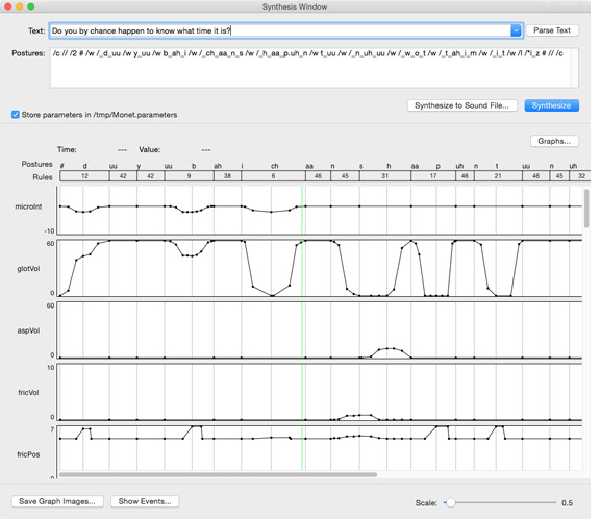
\includegraphics{images/syn-win+line-cursor}
\caption[The ``Synthesis Window'']{\label{syn-win}The ``Synthesis Window'' showing 7 of the 32 parameters for the \newline\emph{first part} of the utterance ``Do you by chance happen to know what time it is?''}}
\end{figure}

Thus the operation of the Synthesis Window is straightforward. The postures field can be edited, and the changed string spoken, to see the effect of different posture selections or changes rhythm and intonation.

\begin{figure}[htb]
{\centering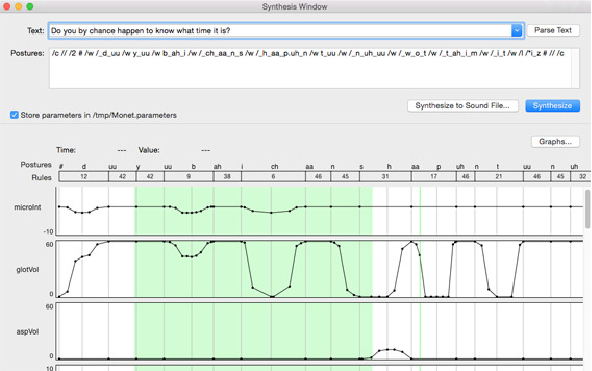
\includegraphics{images/syn-win+line-curs+selection}
\caption[Selected synthesis time extent]{\label{syn-slct} The ``Synthesis Window'' showing a selected time extent and a time line}}
\end{figure}

Apart from the use of the cursor to display the time and value at any point on a parameter track, the synthesis window includes a line cursor (green) running over all the tracks that can be moved to facilitate relating the points in one parameter track to points in other tracks. By clicking the mouse within the tracks area, a line green cursor appears, and can be dragged to any selected time position. Additionally, by shift-clicking and dragging, a time range may be selected for synthesis. Figure \ref{syn-slct} shows both the line cursor, and a selected region. The two facilities are independent. Clicking on a time position moves the line cursor to that position. Holding the mouse button down and dragging allows the cursor to be dragged. Holding the shift key down whilst clicking without moving allows the selected area to be cancelled or, if the mouse is dragged, the selected area is changed to whatever time extent the new shift-click dragging covers.

\subsection
{Intonation and Rhythm}
\label{int-rhythm}

The rise and fall of pitch that  together constitute ``Intonation'' is closely tied to the rhythmic beat of an utterance.  The salient syllables are what Halliday (1970) uses to divide utterances into what he calls ``feet'' (see Appendix \ref{halliday}), each foot beginning with a salient syllable. The perceived rhythm of the speech is dependent on these beat times, whose precise timing is, in turn, are determined by the durations of the sounds generated from the posture sequences when speaking. The feet are grouped into what Halliday calls ``Tone Groups'' of which he defines 5 major varieties, plus two combinations, and a number of finer secondary variants (see Appendix \ref{halliday}). The feet may be: ``pretonic'', leading up to the ``tonic''; or tonic---said to be ``marked'' and are specially lengthened, with the first foot of the tonic receiving the main intonational effects. Utterance final feet are also marked. All postures in a marked foot have longer duration than in umarked feet. Post-tonic feet, those following the tonic up to the beginning of the next tone group or to the end of the utterance, are not marked except for the utterance final foot (which may also be the tonic foot of the tone group. It was found that the rhythm and intonation resulting from this simple model, created on the basis of extensive experiments in the author's lab, was perceived as natural as a more complex model due to Collier and 't Hart and their co-workers 't (for example: Hart \emph{et al.} 1990; Willems \emph{et al.} 1988) in subjective experiments (Taube-Schock 1993).

Our rhythm experiments showed that there were three independent sources of variation in determining the duration of the component postures in feet. Thus these are the basic determinants of rhythm---(1) the posture identity (approximately 45\%); (2) whether the posture was in an marked rhythmic unit---foot---or an unmarked unit (approximately 15\%); and (3) a regression on posture length, decreasing---as the number of postures in a foot increased (approximately 10\%).\footnote{This effect has misleadingly been called ``isochrony'', implying equal length of the feet when the length of different feet is, in fact, merely a little more equal than might be expected, based on the nominal duration of the postures involved. Nevertheless, the effect is important (Hill, Witten \& Jassem 1977, Jassem, Hill \& Witten 1984), and is accounted for by a linear regression that reduces the length of all the postures in a foot in proportion to the number of postures, as the number of postures in the foot increases. The effect is insignificant for unmarked feet but very significant for marked feet.} Thus a total of roughly 60\% of the rhythm of spoken British English for synthesis is accounted for by choosing the durations of the postures according to their marked or unmarked varieties\footnote{This leads to 132 postures comprising marked and unmarked versions of 66 different postures, including silence, rest, and some artificial postures placed by the rewrite rules.} with another 10\%  of rhythm accounted for by the rhythmic unit regression. This allows the SpeechServer to produce articulated speech with roughly 70\% of the rhythm accounted for. This has a very significant effect on the naturalness. The remaining 30\% of the rhythm may well represent free variation, as all of the traditional phonetic correlates of posture duration variation were investigated and found \emph{not} to be independent of the three factors above.

Other intonation experiments we carried out showed, amongst other things, that listeners seem to perceive intonation changes ``categorically''---in the linguistic sense of that word. That is to say there were timing boundaries, and pairs of utterances with intonation changes were only perceived as different if the intonation changes for the members of the pair occured on opposite sides of that boundary (Hill \& Reid 1977). Thus it is important to get the intonation changes in ``the right place'', but provided such boundaries are taken into account, the exact placement is not critical. However, utterances typically have at least one tone group and its associated ``tonic'' foot. The postures in the tonic foot have marked duration, and foot receives a major movement of the pitch, with the tonic syllable---the initial syllable of the tonic foot---having the lion's share. The tonic feet provide the information points of  utterances.

More work is required in these areas. We used a simplified version of Halliday's intonation model for Gnuspeech contours (implementing only statements, questions and emphasis---factors that could be deduced from the punctuation), and implemented rhythm based on: posture identity; whether the posture is marked or not; and how many postures occurred in a marked foot, as well as the location of the beat. Halliday's complete  intonation model is outlined in Appendix \ref{halliday}.

Currently, the tonic for the tone group always defaults to the last foot in the tone group. Some additional parsing (or even better, understanding) could allow the tonic(s) (information point(s)) of the utterances to be placed more intelligently, according to the context for which the utterance is intended. For example, in the utterance comprising a single statement tone group (tone group 1), in answer to a question about ``the killing of John'', the placement of the tonic or information point of the tone group (indicated by  \textsl{\textbf{bold italic}} below) depends on exactly what question is being asked:

\begin{enumerate}
\item{``\textsl{\textbf{Bill}} killed John'' answers the question ``Who killed John?''}
\item{``Bill \textsl{\textbf{killed}} John'' answers the question ``What did Bill do to John?'' and}
\item{``Bill killed \textsl{\textbf{John}}'' answers the question ``Whom did Bill kill?''}
\end{enumerate}

\begin{figure}[htb]
{\centering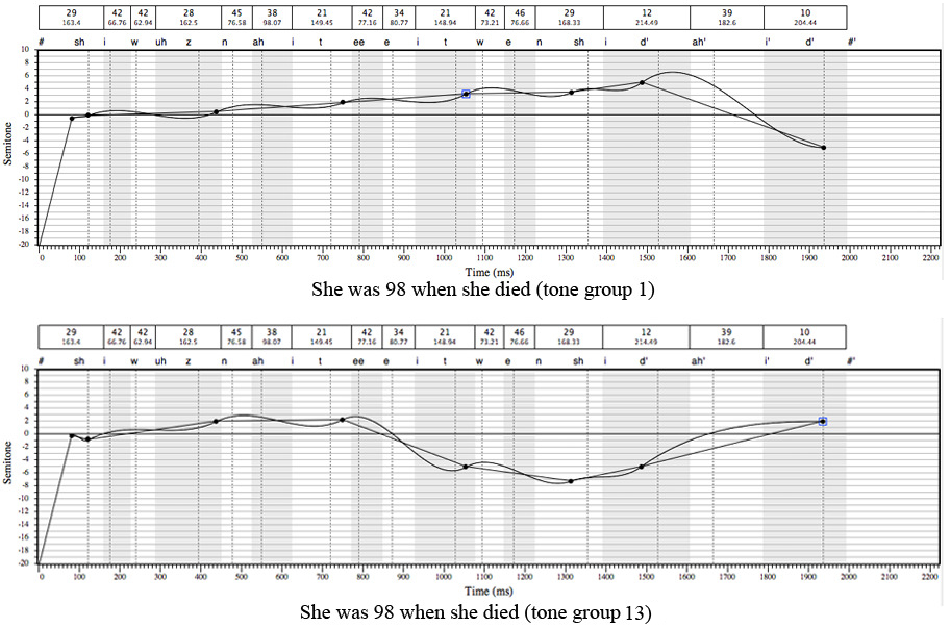
\includegraphics[height=8 cm]{images/she-was-98-comparison}
\caption[Tone Group 1 and 13 comparison]{Comparison of less natural (Tone Group 1) and more natural (Tone Group13) synthetic speech for the utterance ``She was 98 when she died''\label{tgcomp}}}
\end{figure}

\href{https://youtu.be/RefxvPP9UWw}{\underline{{\textcolor{blue}{Listen to a comparison of the Tone Group 1 version followed by Tone Group 13.}}}}

\clearpage

\subsubsection{The intonation parameters \& the intonation window}

\begin{wrapfigure}[25]{L}{0.45\textwidth}%This example of wrapfigure is from
\vspace{-20pt}% Donald Arseneau's article ``The wrapfig package'' 2003-01-31
\begin{center}
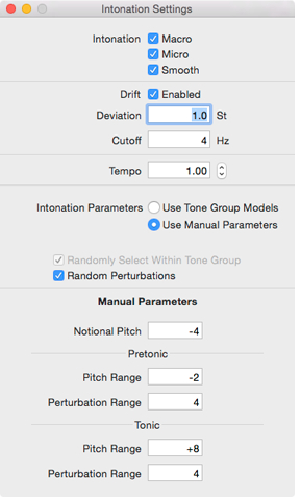
\includegraphics[width=.4\textwidth]{images/intonation-settings-for-int-win-fig}
\caption{\label{int-par2}The manual intonation settings}
\end{center}
\vspace{-20pt}
\vspace{1pt}
\end{wrapfigure}

Figure \ref{int-par2} shows ``Intonation Settings'' window that produced the intonation contour portrayed in the full ``Intonation'' window shown as Figure \ref{int-win}. The check boxes at the top show that all the options were enabled. ``Macro" refers to the basic intonation contour; ``Micro'' enables microintonation;  ``Smooth'' applies a simple curve fit to the contour (which needs to be improved); and ``Drift'' currently does little and is a historical relic. ``Tempo'' allows the rate of utterances to be change---1.00 represents normal speed with fractions being slower and \textgreater{} 1.0 being faster. ``Random Perturbations'' applies random changes to the value of points defining the intonation contour to provide variety when repeating the same utterance.

The intonation parameters used may be selected as ``Use Tone Group Models'' or ``Use Manual Parameters'' using the radio buttons. In the latter case the manual parameters that control the ``Notional Pitch'', the range and perturbations of the pretonic, and the range and perturbations of tonic may be entered as positive or negative floating point values. The Notional Pitch determines the pitch at which the intonation contour starts within the two octave range from -24 to +24, with zero being Middle \textquoteleft{}C' (261.626 Hz). The remaining four parameters use positive values for a rise and negative values for a fall. When ``Use Tone Group Models'' is selected, the manual parameters are greyed out and ineffective whilst ``"Randomly Select Within Tone Group'' becomes active, and uses the basic tone group models, but allows both pretonic and tonic point values and ranges to be varied somewhat from their nominal values in successive utterances.


\begin{figure}[htb]
\centering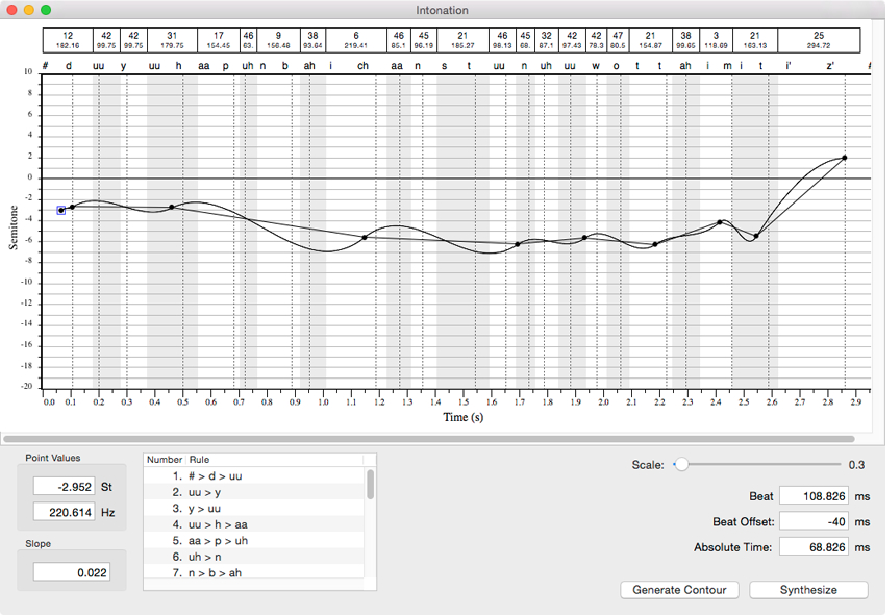
\includegraphics{images/intonation-window-new}
\caption{\label{int-win}The full intonation window}
\end{figure}

An utterance to be synthesised is entered into the text field of the Synthesis Window  and parsed (see Figure \ref{syn-win}). The Synthesise button produces the spoken version. There is also a Synthesise button in the Intonation window which also produces a spoken version. However, the two buttons have somewhat different uses and effects and will be referred to as ``Synthesise-1'' and ``Synthesise-2'', or ``S-1'' and ``S-2'' for short.

S-1 always speaks based on generating an intonation contour for the utterance either according to  the settings from the models---perhaps with random perturbations, or according to the manual settings, depending on which radio button was active. S-2 always generates a spoken utterance using the contour that is on display, which can be one previously generated by S-1, or one produced by clicking the ``Generate Contour'' button on the Intonation window; or it can be one that was modified from a previously generated contour. Points defining the contour may be added, or deleted, or moved. To add a point, Option-click at the time the point is required---the point will appear at the time and value position of the cursor, dragging the contour towards itself as necessary.

To move or delete a point, first ``lassoo'' it by dragging the cursor across it. Hitting the delete key removes it. Using the arrow keys moves it in increments---a semitone at a time in value---up or down, or by a distance related to the posture structure in time, forward or backward. A red line appears if the forward or backward changes moves the point on top of another point.

To achieve finer positioning in frequency of a selected point, the semitone value or Herz value may be entered in the appropriate field under ``Point values'' at the bottom left. To achieve finer positioning in time, a point can be added at whatever time is required, positioning the cursor on the scale at the bottom when clicking, and then repositioning the point to whatever frequency value is required.

The slope field is not currently very useful or informative and can be ignored for now. The sub-panel on the right of the Point Values shows all the rules that were used in the composition of the postures. The extents of the rules are marked on the plot of the intonation as stripes alternating between white and grey. The dotted lines represent potential beat locations for the utterance, which are identified along the top edge of the plot. Above that, registered with the stripes, are the rules and the rule durations. A scroll bar underneath the plot allows an oversized plot to be scrolled. If it is not visible, just increase the height of the window a little and it will appear. There is also a ``Scale'' slider just below the scroller, on the right. If the scale is reduced to accommodate a longer contour, some of the rule durations may overlap and become unreadable. Enlarging the scale and scrolling to the area concerned allows the information to be seen

At the bottom right corner are fields displaying the ``Beat time'', the ``Beat Offset'' and the ``Absolute Time'' of the point selected. If no point is selected, these are blank. They are not editable (but they perhaps should be, to facilitate the absolute time positioning of a selected point). Below those fields two buttons are placed: ``Synthesize'' (S-2) which has already been discussed and ``Generate Contour'' which generates the same contour as would be generated by clicking S-1.

When synthesising from the ``Synthesis'' window, the basic macro contour form is generated (no smoothing) and the contour displayed varies in value, even when all six check boxes at the top are unchecked. However, the speech output is monotone, as required. It is debatable as to whether the contour should be a straight line, with the points still shown. The contour that is produced varies appropriately according to which of the two radio buttons is activated. If ``Use Tone Group Models'' is active, the ``Manual Parameters" lower down are inactive and greyed out. Also the ``Randomly Select Within Tone Group" is active and may be checked if desired. The effect of this is to change the notional pitch, the pretonic slope, and the tonic slope within the basic tone group framework. Selecting ``Random Perturbations" adds random displacement of the contour points for both the radio button selections. These displacements can be large enough to change the perception of the tonic---audible competition if ``Macro'' has been checked to produce non-monotone speech. This is not a good feature.  The drift parameters are greyed out if the "Drift" box is unchecked, but Drift is not currently relevant.

If ``Use Manual Parameters'' is active, then the Manual Parameters are active and not greyed, and the contour shows the effect even though the intonation of the speech output is monotone. The ``Randomly Select Within Tone Group" selection is greyed out and inactive in this condition.

Note well, that the foregoing applies to synthesis using the S-1 button. If the S-2 button in the Intonation window is used, then the intonation applied always follows the contour on display.

``Generate Contour'' always generates a new contour matching the contour that would be generated if the Synthesis window S-1 button were pushed.

It may be noticed that going for the Randomly Select Within Tone Group speech, with Smooth checked, produces a fairly flat version of the contour, just pretonic and tonic in straight lines. Adding smoothing actually does the opposite of smoothing. What it really does is to introduce another source of variation, but it does avoid sharp corners (first and second order discontinuities) in the contour. A better term for what ``Smooth'' does might be summarised as ``Wavy''. A more appropriate smoothing algorithm may be appropriate, though it is hard to hear any difference between smoothed and unsmoothed contours when Macro is enabled, except that if excursions become large enough they may affect the perception of the contour.


\clearpage

\section{Database creation and modification}
\subsection{Preamble}
The Monet database editor is described in what follows as if it is fully working, which it is not quite---yet. The port, well under way, needs to be completed. However, the guide is not only intended as a manual for the use of the system, but also a guide for the completion of the port and further development. The approach is intended to provide insight into the real value of Monet as a linguistics tool---beyond the task of articulatory synthesis. The Speech Server itself is fully functional, independent of the database editor, and the parts of Monet that use the Speech Server for synthesis \emph{are} complete.

\subsection{Getting started}
\label{start}

\begin{wrapfigure}{L}{0.45\textwidth}
\centering{
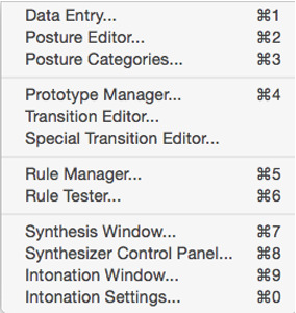
\includegraphics[width=0.4\textwidth]{images/tools-menu-rev}
\caption{\label{tools}The Gnuspeech ``Tools'' menu}}
\end{wrapfigure}
The major subsystems in Monet corresponding to the above divisions/functions, and accessible from the ``Tools'' menu in the bar at the top of the screen and reproduced as Figure \ref{tools}.

When developing a new database, or modifying an old one, the parameter computations necessary for synthesis are carried out ``on the fly'' (i.e. in real time) based on whatever elements of the databases are available at the time. Thus the Monet system may be used to create a new database file as well as to audit and edit existing database files. The following descriptions refer to the existing English database, as defined in the file ``Diphones.mxml'' as noted below in this section.


\begin{wrapfigure}{L}{0.45\textwidth}
\centering{
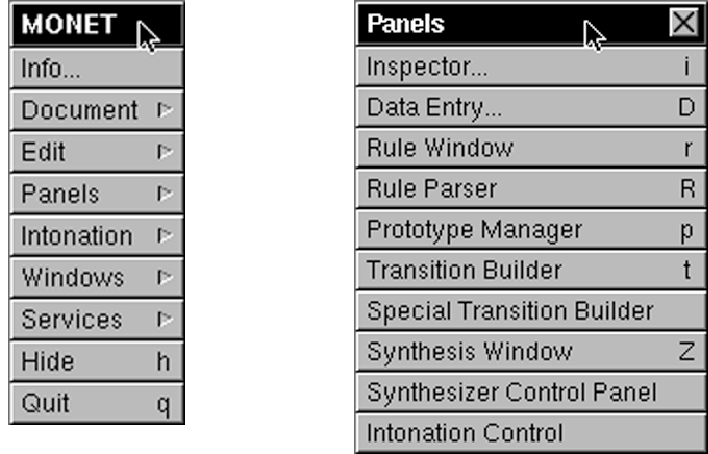
\includegraphics[width=0.4\textwidth]{images/next-main-n-panels}
\caption[GNUStep ``Main'' and ``Panels'' menus]{\label{gnu-panels}The  ``Main'' and ``Panels'' menus: GNU/Linux GNUStep}}
\end{wrapfigure}

If you are using Gnuspeech under GNUStep on a GNU/Linux system, you will see the ``Main'' menu and can then select the ``Panels'' menu, as seen in Figure \ref{gnu-panels}. \emph{However, in that case, this manual is not the right manual for what you want to do}, because the interface for the GNUStep version of Monet is significantly different to the Macintosh version. \emph{This manual is for the Macintosh version}.

It is assumed that you have installed Monet on your system. If you intend working on an existing database, you need to install the database file you wish to work on in the Monet application ``Resources'' folder. If you intend working on the file supplied with the application, you should also make a back-up copy in a safe place. So ``Control-click'' on the Monet application and choose ``Show Package Contents'' from the pop-up menu that appears to show the ``Contents'' folder. In that folder you will find several items, one of which is ``Resources''. Look in that folder and you should find a file named ``Diphones.mxml''. That is the file you should back up if you will be modifying it; or move and then insert an empty template file from ``Documents\textgreater{}Monet'' if you wish to create a completely new database. (The supply of templates for creating a new database has yet to be created.)



The main dictionary, if you need to alter it, is located in:

\vspace{-12pt}

	\begin{center}\noindent{}Frameworks\textgreater{}GnuSpeech.framework\textgreater{}Resources\textgreater{}2.0eMainDictionary.dict\end{center}
\newpage
\vspace{-12pt}
\noindent{}along with the list of suffixes for extending the reach of the dictionary by allowing compounds involving the suffixes to be found. For a language other than English, these will need to be replaced.



Most of the facilities you require to create and modify databases are accessed via the ``Tools'' menu selection (see Figure \ref{tools}). However, to work on a language other than English you will need to modify other components, including the ``Parser'' in the Speech Server. This module is a pre-processor that converts items such as numbers, dates, special characters, possessive ``'s'', and other such items into conventionally pronounceable form. As this is built into the Monet code (it should be made more accessible so that recompilation is not needed), you will need to change some of the Monet code and recompile using the Macintosh xcode development tools if you wish to change the Parser. Initially it can perhaps be ignored, but the task of creating a new language needs to be made much easier.

\subsection{Creating/editing the database}
\subsubsection{Categories, Parameters, and Basic Timing Framework}

The Data Entry window allows the basic posture Categories, Parameters, Meta Parameters, and basic Formula Symbols to be defined. Figure \ref{data-entry-1} shows a partial window with ``Categories'' selected, overlapped by a full window with ``Parameters'' selected. The Categories selection allows categories into which postures might fall to be defined.The categories can used, in parallel with individual posture names, when specifying the composition rules used to process posture strings in order to create the synthesiser parameters tracks needed to speak the utterance. It is a way of generalising what would otherwise be rather specific rules, and cuts down on the number of rules. It is coincidental that there are 16 categories as well as 16 parameters. Categories may be added and deleted, and comments may be supplied. The menu selection ``Posture Categories'' provides a window showing to which categories each posture belongs (a posture may belong to several). The comment at the bottom notes that the category ``phone'' cannot be deleted.

The Parameters selection allows the parameters required for the synthesiser to be defined, as well as their minimum, maximum, and default values to be set. Comments can be added for each parameter. Parameters may also be added or removed using the buttons at the bottom right.

\begin{figure}[t]
\centering
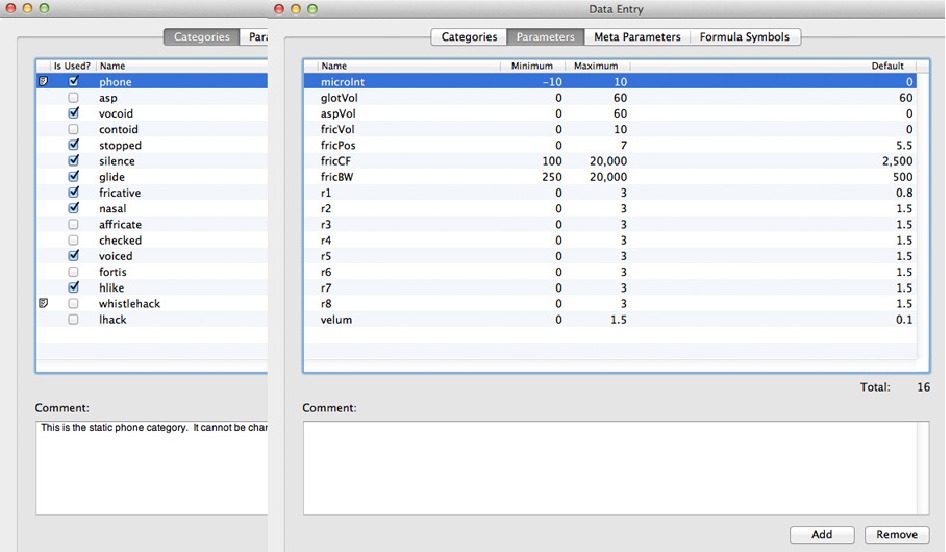
\includegraphics{images/data-entry-categories-n-params-m}
\caption[Data Entry ``Categories'' \& ``Parameters'']{Two Data Entry windows  ``Categories'' \& ``Parameters'' selected}
\label{data-entry-1}
\end{figure}

Figure \ref{data-entry-3} shows a portion of the same data entry window but this time with ``Formula Symbols'' selected. The symbols shown and specified are used as the basic time framework for compositing the posture parameters. The Minimum, Maximum, and Default timing values are specified. Additional symbols may be defined in terms of these basic symbols, plus the timing values derived from posture data, using the ``Equations'' selection in the ``Prototype Manager'' (Figure \ref{pro-man-equ-fig} in section section \ref{pro-man-equ}). These are then used to define detailed timing in the rule-based posture composition process.

\begin{figure}[t]
\centering
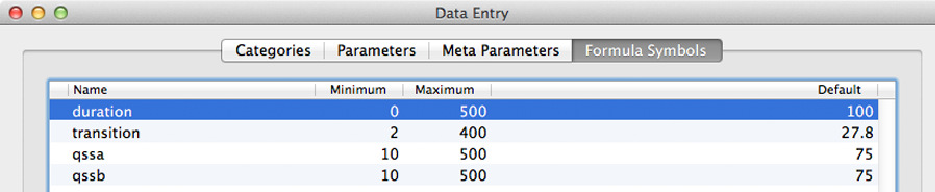
\includegraphics{images/data-entry-formula-symbols-crop}
\caption[Data Entry ``Formula Symbols'']{Data Entry window ``Formula Symbols'' selected}
\label{data-entry-3}
\end{figure}

\subsubsection{Posture Editor}
\begin{figure}[htb]
\centering{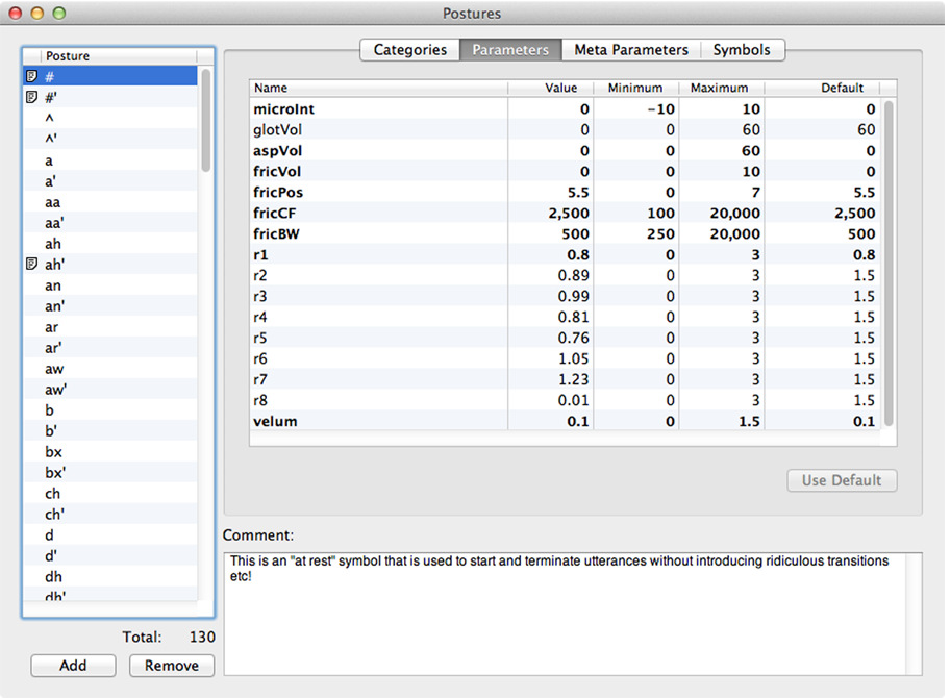
\includegraphics{images/postures-parameters}
\caption[The Postures window]{The Postures Parameter entry window
\label{pos-ed}}}
\end{figure}

Figure \ref{pos-ed} shows the ``Postures'' window that allows postures to be added, edited and removed. To add a posture, click on ``Add'' then enter the name of the new posture and hit Return. The posture will move to its correct position in alphabetical order. Find it and click once on the entry (if you double-click you can change the name). With the name highlighted you can use the selections ``Categories'', ``Parameters'', ``Meta Parameters'', and ``Symbols'' to enter those data for the new posture. If starting from scratch, the window will already have ``phone'' as a category (supplied by the template you obtained), but other appropriate categories can be added by clicking the appropriate boxes. The parameters will be set to default values but can be changed by selecting Parameters, double-clicking the specific parameter value, entering the required value, and hitting Return.\footnote{The basic Parameter targets specify the nominal values needed to drive the synthesiser to realise each posture. For our articulatory synthesiser database these include: cross-sectional radii, r1 through r8; the state of the velum; specification of superimposed microintonation; and so on, as shown in Figure \ref{data-entry-1}.} Meta Parameters are not yet used but will operate in a similar fashion. The Symbols selection allows different posture timing to be entered, based on changing the default values that have already been entered, by double clicking the value, entering the new value and hitting Return. Which of the symbols is used, and in what portion, is determined by the composition rule that gets selected when a string is composited, but the ``duration'', and ``transition'' times are nominal values for the quasi-steady-state duration and the transition to and from the posture quasi-steady-state, whilst ``qssa'' and ``qssb'' represent the division of the quasi-steady-state into nominal first and second portions. How they are actually used depends, as noted, on the applicable composition rules---and their associated equations (see Section \ref{equations}).


\subsubsection{Prototypes, Equations, and Transitions}
\label{intonation}
The data needed to make the entries described must be supplied from phonetic analysis of natural speech in the target language and dialect, augmented by published data. Separating the components for transition and quasi-steady-state portions requires judgement and insight. The process is not strictly a traditional phonetic analysis which tends to lump transitions with the overall duration of ``vocoids'' (open sounds with little constriction). The transitions between two postures will frequently be dominated by one of the postures---for example, the stop-to-vowel transition in English depends mainly on the stop rather than the vowel, though the details may depend on both. The composition rules and transition prototypes  (see Sections \ref{rule-man} and \ref{transitions}) have to be designed with these constraints in mind, plus the fact that the transitions may start and end at different times for different parameters.

The posture data and rules then require evaluation on the basis of speech synthesised using the database being built. This process involves both spectrographic analysis of the synthetic speech and careful listening trials which initially may be informal, but ultimately require formal subjective-test evaluation.

In the current database for English, there are 132 posture variants (2 x 66 as previously noted). Some are closely related to conventional phonemes whilst some are special postures, added by rewrite rules (see Appendix \ref{rewrite}), that are applied in the preprocessing, along with the parsing of numbers and so on. The large number results from the rhythm studies and the design of the intonation and rhythm models. (see section \ref{int-rhythm}).


\subsection{Prototype Manager and Transitions}
\label{pro-man-equ}
Figure \ref{pro-man-equ-fig} shows the Prototype Manager. Three selections may be made: Equations, Transitions, and Special Transitions
\label{equations}
\subsubsection{Equations}
With ``Equations'' selected, as in Figure \ref{pro-man-equ-fig}, named equations may be created to define event times, in terms of the basic named time symbols of postures. They may be grouped. New named groups may be created. Both equation names and group names should be designed to indicate the nature of the association of the group members and the purpose of event times corresponding to the named equations. The named event times are used to determine where changes will occur when creating Transitions and Special Transitions. The event times determined by the equations are created as needed. Superfluous equations may be removed.

By defining some timing symbols in a regular succession, points in the Transition Profiles may be systematically moved by selecting different symbols for successive synthesis trials of a given utterance. In this somewhat tedious manner, systematically varying stimuli may be produced for various purposes, such as psychophysical experiments (e.g. voice onset time experiments). The system should be provided with more (semi-)automated tools to facilitate the kinds of time and other changes needed for such work.

\subsubsection{Transitions}
\label{transitions}
\begin{figure}[htb]
%\centering
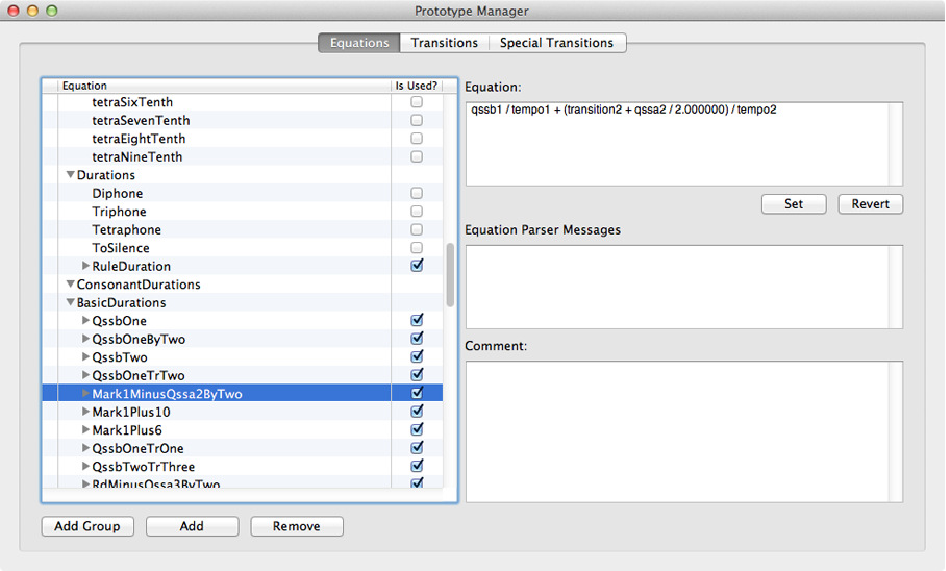
\includegraphics{images/prototype-manager-equations-Mark1MinusQssa2ByTwo}
\caption{\label{pro-man-equ-fig}Prototype Manager: Equations}

\end{figure}

\begin{figure}[htb]
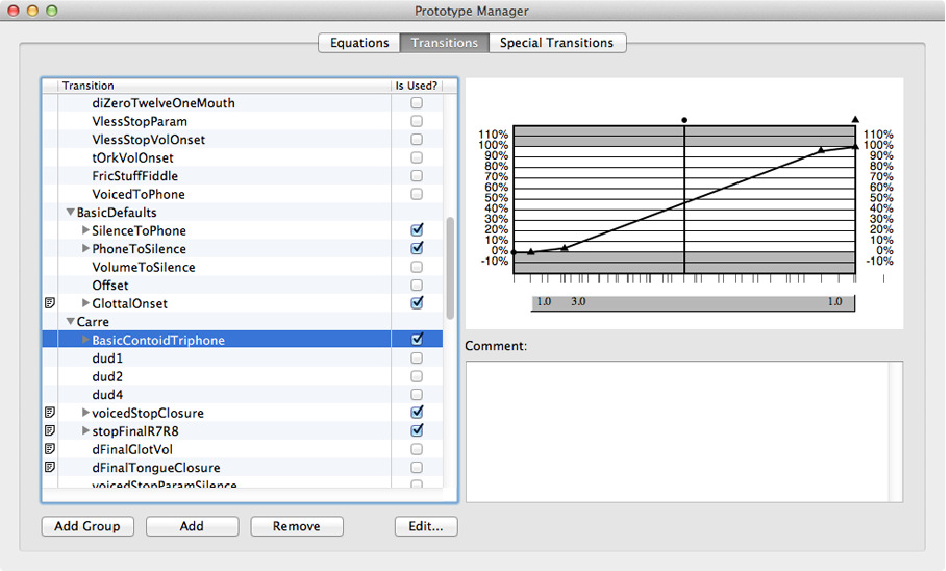
\includegraphics{images/carre-basic-contoid-triphone}
\caption{\label{pro-man-tran}Prototype Manager: Transitions}

\end{figure}

Figure \ref{pro-man-tran} shows the same prototype window, but with Transitions selected. The particular transition on display is ``BasicContoidTriphone'', that is put in the Carr\'e group of transitions. The shape of the points on transition graphs indicate the segment to which the transition leads. A ``{\Large\textbullet}'' leads to the second target, a ``$\filledmedtriangleup$''  to the third, and a ``$\filledmedsquare$'' to the fourth (as in a tetraphone). Note that this triphone actually ignores the second target and thus only has ``$\filledmedtriangleup$'' symbols showing.

Slope ratios are generally used to control the transition shape by defining the relative slopes in the (ordinary) ``Transition Prototype'' because of the way the parameter transition shapes are converted into actual parameter tracks. Unlike the Special Parameter Transitions---where the requirement is simply to add an absolute value excursion onto the particular parameters track---with the normal transitions it is necessary to apportion the amounts of change that are to take place in the successive segments of the transition \textit{without knowing (at the time the transition prototype is constructed) what the absolute time or change in value will be}. That is to say, the same prototype shape, which is the important aspect of the normal transitions, has to apply to a variety of time and value changes. This is also related to why the last point of an \emph{n}-phone is a phantom point---you can't generate the complete actual transition until you have the next \emph{n}-phone target to give you the actual value that determines the absolute change that will be apportioned according to the slope ratios for the transition.

As noted, slope ratios are \emph{not} used for  ``Special Transition Prototypes'' since they are simply excursion superposed on the basic shape determined by the Transition Prototype. Focussing on the shape of transitions is an effective method of modelling the constraints of the articulators without having a physiological model with all the muscles, masses, joints and so on.

The left-hand column shows whether there is a comment associated with a given transition (none are shown in Figure \ref{pro-man-tran} or related figures. The box on the right of the names tells whether the transition is actually used in a composition rule or not. The comments are displayed in the lower field on the right (accessing and displaying the comments that exist does not currently work).

The transition shape and timing points are displayed in the upper field on the right, time progressing on the \emph{x}-axis and percentage of the total change demanded on the \emph{y}-axis. Note that and extra 20\% of the range is allowed in case it is necessary to define an under- or overshoot of the target's nominal value.

\begin{figure}[htb]
\centering
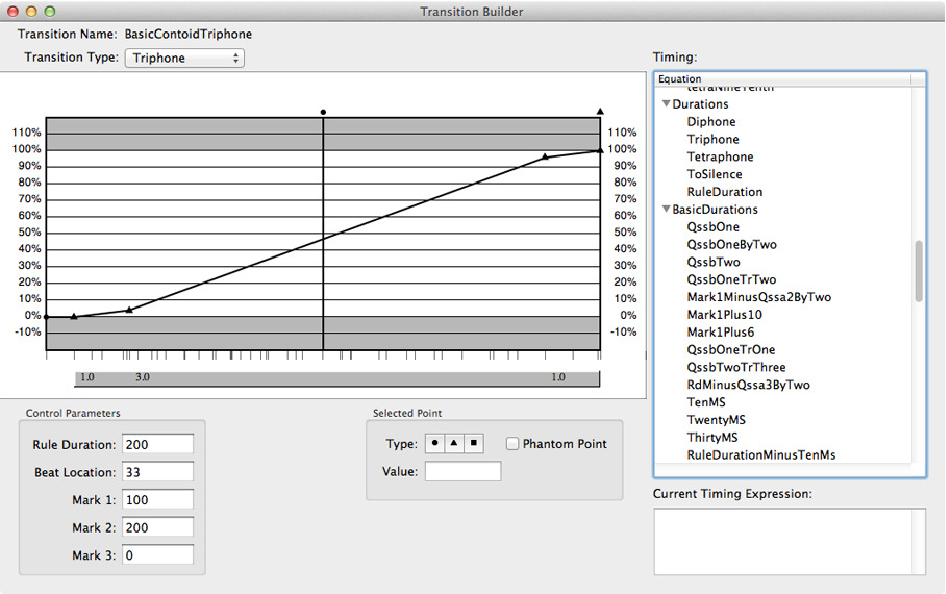
\includegraphics{images/transition-builder}
\caption{The Transition Builder window}
\label{tran-bld}
\end{figure}



In order to edit the transition, the user needs to click on the ``Edit'' button which brings up the Transition Builder window shown in Figure \ref{tran-bld}. The time position of a given point may be changed by selecting the point (drag across it to lasso it, when it becomes surrounded by a lightly drawn square), and then selecting a different event time from the list on the right-hand side. To change the shape of the  transition, click on the numbered area below the transition where the slope ratios are displayed. The selected slope ratio become editable, with the range to which it applies obvious from the highlight that replaces the grey field. Note that when a slope ratio is changed, all the segments that are determined by slope ratios are changed, since the total change will now be apportioned differently when the actual parameter values are computed for the specific targets involved in generating the parameter track for the parameter(s) to which the transition applies. This is shown in Figure \ref{tran-bldr-slp-chng} which shows just the relevant part of the Transition Builder window during and after a fairly extreme slope ratio change to the second segment of the BasicContoidTriphone transition that was originally seen in Figure \ref{tran-bld}.

At present it is not possible to remove a transition that has been built even though a button for that is provided. For this reason there are a number of ``dud'' profiles, usually numbered to distinguish them, with ``dud'' indicating that they are \emph{not} good transitions so as to avoid confusion during database creation. Obviously this needs to be changed.


To create a new transition, the ``Add'' button in the Prototype Manager button should be clicked. A new ``Untitled'' entry will appear in the list of transitions. Enter an informative name in the style typified by existing entries (i.e. ``camelCased''\footnote{Camel casing is the practice of writing compound words or phrases such that each successive word or abbreviation begins with a capital letter. \emph{Camel case may start with a capital or, especially in programming languages, with a lowercase letter.}}). Hit return, then click ``Edit'' whilst the new entry is highlighted. A Transition Builder window will open showing a linear diphone transition will appear. The pull-down menu below the new transition name at the top left can be used to change to a triphone or tetraphone. Points may be added by double-clicking, and then choosing the correct type (``\textbullet{}'', ``$\blacktriangle$'', or ``$\blacksquare$''). The percentage position of the added points may be changed by lassooing the target point and entering the value. The time position may be changed by selecting the equation defining the desired new event time from the list on the right-hand side. This where the process of creating transitions can get derailed and confused, as there is no ``Undo'' button---obviously one should be added. At present, the bad transition must simply be renamed ``Dud\emph{n}''.

\begin{wrapfigure}{L}{0.5\textwidth}
\centering
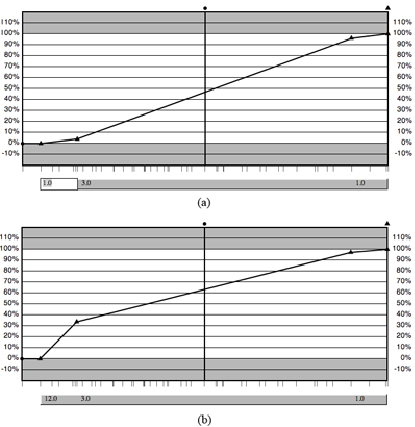
\includegraphics{images/tran-bldr-slope-change}
\caption{Changing a transition shape}
\label{tran-bldr-slp-chng}
\end{wrapfigure}

At the final boundary it will be necessary to mark the  point that defines the end of the transition segment as a ``Phantom'' point (as discussed above). There is no apparent reason why this should not be automated. As noted, the transitions provide appropriate change trajectories for the different posture parameters in particular phonetic contexts to replicate the movements associated with articulation. It can be helpful to have identical transitions with different names associated with different rules/contexts. For this reason a ``Duplicate'' or ``Alias'' button would also be useful to provide access to the same transition via a different name (saving storage whilst improving the human-computer interface).

The timing values that control the current transition segment are displayed at the bottom left of the window. Since the shape of the transition is independent of the times and values of any specific posture combination, the display is only for mis-information (!) and is not currently activated---the same values are always displayed and changing them has no effect. The actual timing is determined by the selected event times computed from the timing associated with each posture and the current ``Tempo''; and the absolute values of the parameters depend on the posture targets perhaps modified in both timing and value modified by the transition prototype.

In order to apply slope ratios to two or more transition segments in a new transition it is necessary to select all the points that define the endpoints of the segments by Shift-clicking them in turn, or lassoing them all at once. When all are selected the button ``Apply Slope Ratios'' should be clicked. A new set of fields will appear beneath the transition, initially with each slope ratio set to 1.0. Clicking on one of the fields will highlight the selected ratio, with the visible field showing the extent of the segment that is about to be changed, as describe at the beginning of this section. The port for this facility has yet to be completed. Saving changes is not yet implemented.

\begin{figure}[htb]
%\centering
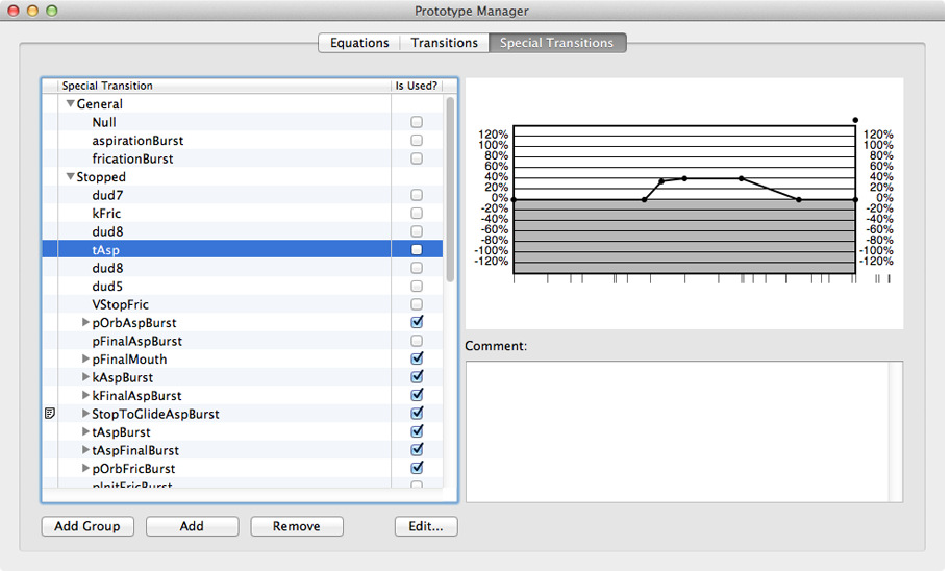
\includegraphics{images/prototype-manager-special-transitions-tAsp}
\caption{Prototype Manager: Special Transitions}
\label{prot-man-spec-tran}
\end{figure}

\subsubsection{Prototype Manager: Special Transitions}

The creating, editing and removing Special Transitions is very similar to the procedure used for Transitions except that slope ratios are not applicable.


\subsection{The Rule Manager}
\label{rule-man}
\begin{figure}[htb]
\label{rule-man-fig}
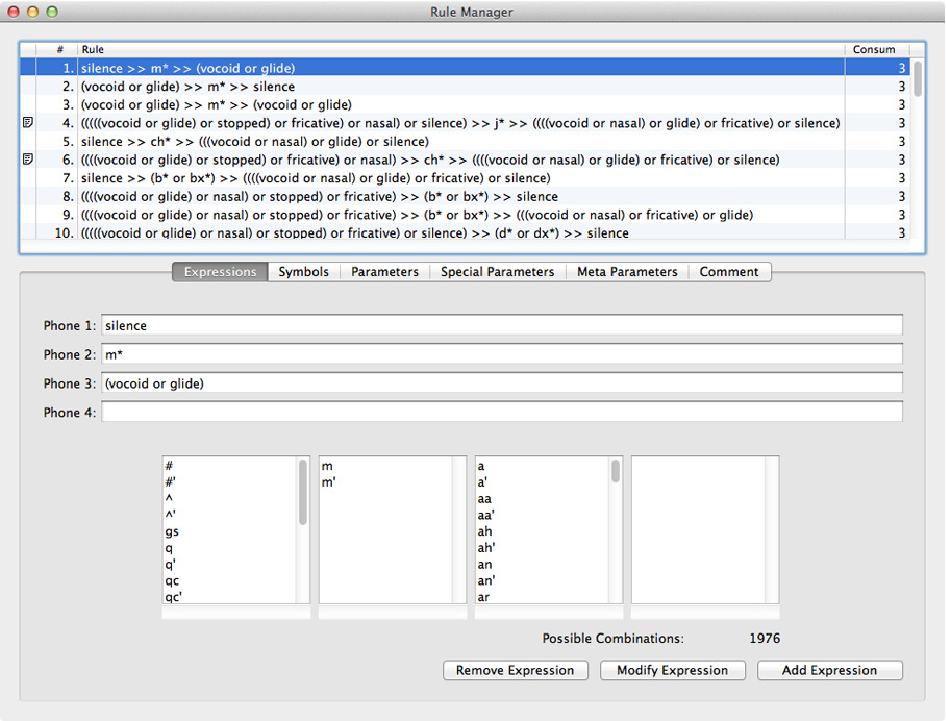
\includegraphics{images/rule-window-expressions}
\caption{\label{rul-man-exp}The Rule Manager: Expressions}

\end{figure}

\subsubsection{Introduction}

Figure \ref{rul-man-exp} shows the Rule Manager window with ``Expressions'' selected. These are often called ``The Rules'', and can be identified individually as ``Rule \emph{n}''. Each rule represents a posture combination and will determine which transitions will apply to each parameter transition for each sequence of postures covered by the rule, leading to the composition of a further segment of the parameter tracks. There are currently 47 rules, including ``phone\textgreater{}\textgreater{}phone'', a rule which is always the last rule and cannot be moved or deleted. Other rules \emph{can} be both moved and deleted. The order is important in order to make sure that the more specific rules are applied before more general rules.

The rules are tried, starting from the top rule, and proceeding down towards the last rule until a rule that ``fits'' a portion of the current posture string, starting with the last posture used, is found. Thus the rules should be organised from the most specific at the top to the most general at the bottom (phone\textgreater{}\textgreater{}phone)

Applying a rule to a set of postures may involve some rewrite rules.

\subsubsection{Expressions}
Selecting Expressions allows an expression comprising two, three or four postures to be entered. Each posture may be specified explicitly by using a specific posture symbol, or as a category, or as a logical combination of categories and postures. Consider Rule 7:

\vspace{6pt}
(silence) \textgreater{}\textgreater{}(b* or bx*) \textgreater{}\textgreater{}((((vocoid or nasal) or glide) or fricative) or silence)

\vspace{6pt}
\noindent{}Posture 1 is Silence. Posture 2 in the sequence can be a  /b/ or /bx/\footnote{An ``asterisk'' (*) indicates a marked or unmarked posture---marked postures have a ``prime'' (\textprimstress).}, and item 3 can be any single posture from the categories: vocoid, nasal, glide, fricative, or silence. The second silence seems redundant because silence b* or bx*\textgreater{}\textgreater{}silence is not likely, but complete coverage of possible inputs is important.

The individual postures sequences that are covered by the rule are listed in columns below for convenience along with the number of legal combinations of postures. Note that Figure \ref{rul-man-exp} relates to rule 1, not to rule 7. Expressions may be added, modified or removed using the appropriate buttons. To modify an expression, the components should be entered in the Phone 1 to Phone 4 fields, and then the ``Modify'' button selected. At present changes to the database cannot currently be saved because saving in the GUI-based database editor is disabled. This is true of all the changes that could be made, including those using the Rule Manager.

\subsubsection{Symbols}
When ``Symbols'' is selected, the named timing values determining the basic framework according to the selected equations are displayed in the bottom left portion of the window as shown in Figure \ref{rul-man-sym} which presents a cropped portion of the Rule Manager window.

\begin{figure}[htb]
%\centering
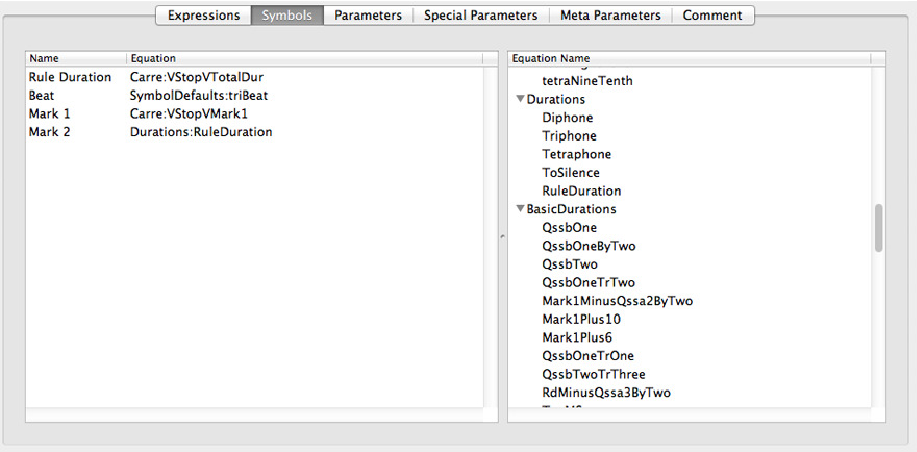
\includegraphics{images/rule-window-symbols-crop}
\caption{The Rule Manager: Symbols}
\label{rul-man-sym}
\end{figure}

A different equation may be used to determine these timing values of a given (selected) rule by highlighting the value to be changed, finding the desired equation in the list on the bottom right, and double clicking it. If a new equation is needed it is necessary to go to the Prototype Manager (see Section \ref{equations}) and create it. It will then show up in the ``Equation Names'' in the Rule Manager window where it can be selected as just described. Again, this aspect of the port remains to be completed. The nature of ``Beat'' is explained in Section \ref{beat}.

\subsubsection{Parameters}
\label{params}
\begin{figure}[htb]
%\centering
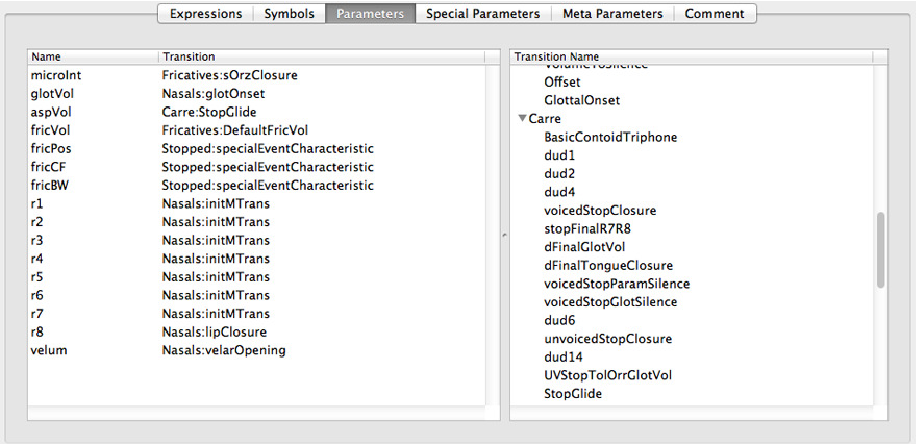
\includegraphics{images/rule-window-parameters-crop}
\caption{The Rule Manager: Parameters}
\label{rul-man-par}
\end{figure}

Figure \ref{rul-man-par} shows the bottom portion of the Rule Manager when ``Parameters'' has been selected. On the left are the names of the parameter Transitions that govern each of the regular parameters for this rule. Highlighting a parameter and double clicking a ``Transition Name'' on the right-hand side causes the selected transition to be used to govern the transition(s) for that parameter. The updated Transition Name replaces the one that was in place for the parameter previously. If a new transition is required, it is necessary to create it first, using the Prototype Manager and the Transition Builder as discussed above (see Section \ref{transitions}).\footnote{The Tools menu item shows ``Transition Editor'' instead of ``Transition Builder'', but should not be invoked by that path anyway. The same applies to the ``Special Transition Editor'' selection referencing the ``Special Transition Editor''. At present, the transition that comes up is an unalterable blank.} Note that each parameter can have a different transition graph specified for each of the 47 rules.

The transitions are created according to linguistic knowledge, coupled with analysis of relevant synthesiser output, produced in the various contexts covered by the rule that is involved, using a high quality spectrographic analyser as well as informal listening trials by native speakers. When some success in synthesis has been achieved, formal subjective listening trials are called for.

The porting for this facility remains to be completed but much of the work is done.

\subsubsection{Special Parameters}
\label{spec-trans}
\begin{figure}[htb]
%\centering
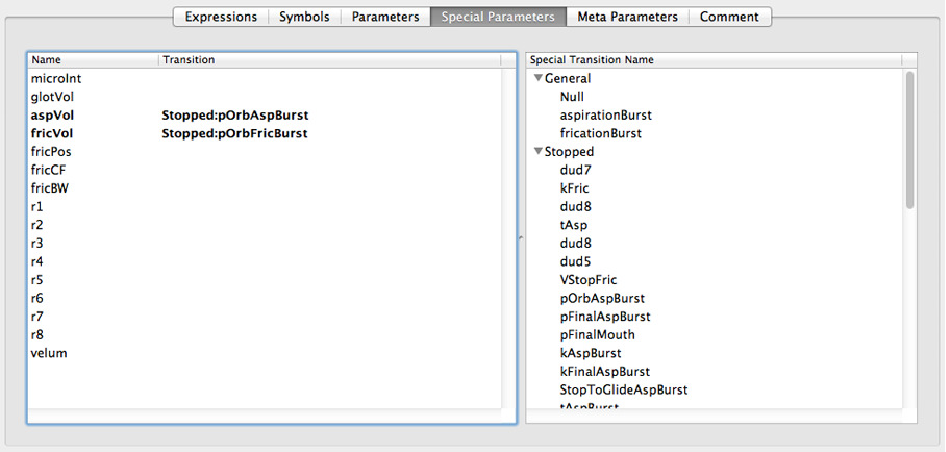
\includegraphics{images/rule-window-special-parameters-crop}
\caption{The Rule Manager: Special Parameters}
\label{rul-man-spec}
\end{figure}

Figure \ref{rul-man-spec} shows the bottom portion of the Rule Manager window with ``Special Transitions'' selected. The Special Parameters use the Special Transitions created using the Prototype Manager and the Special Transition Builder.\footnote{Note the previously mentioned Tools menu name problem.}
The procedure is very similar to what was described for the Transition parameters management (Section \ref{params}). However, since these are special transitions, it is only necessary to enter the transitions that actually occur. They are then applied by adding them to the basic parameter transition during parameter track generation. In the example shown only excursions of ``fricVol'' and ``aspVol'' are required to provide noise bursts for the \emph{n}-phone rule involved. The Special Transition can be set or changed by double clicking the appropriate name in the list of Special Transition Names in the list at the bottom right. If a new Special Parameter Transition is needed, it will be necessary to use the Prototype Manager and the Special Transition Builder to create it (see \ref{spec-trans}). It will then become available in the list for the Rule Manager: Special Parameters: Special Transition Name and can be selected.

\subsubsection{Meta Parameters and Comments}
The Meta Parameters selection currently does nothing, because no framework for handling Meta Parameters has been formulated. The selection is provided for future implementation when such parameters have been formalised (for example, jaw rotation and tongue height could be used to estimate selected tube radii; lip opening would affect R7 and R8, probably as modified by jaw rotation).

The comments window applies to all the selections to allow suitable comments to be added to document the reason(s) for a given choice, to note any special conditions, etc.

\subsubsection{The Rule Tester}
\begin{wrapfigure}{R}{0.5\textwidth}
\centering
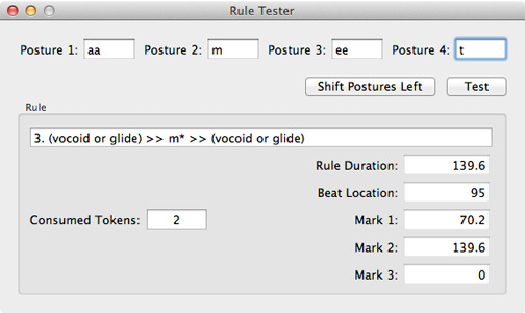
\includegraphics[width=0.4\textwidth]{images/rule-tester}
\caption{The Rule Tester}
\label{rul-test}
\end{wrapfigure}

The ``Rule Tester'', shown in Figure \ref{rul-test} allows the user to enter a sequence of postures to see which rules will apply during composition. When a sequence of postures has been entered, clicking the ``Test'' button shows which rule would apply to the postures and the number of postures used for the rule, starting at the left-hand end. The postures can be shifted left, keeping the unconsumed tokens left over from the previous rule, and further postures entered.

Currently the tester does not distinguish between  marked and unmarked versions of the postures and will therefore not operate correctly to distinguish two rules that differ only in whether marked or unmarked postures are involved---if there were such rules. The notation in the rules showing an asterisk (*) against a posture indicates that either a marked or an unmarked posture is acceptable. A prime (\textquotesingle) indicates a marked version

The basic timing parameters for the rule, Rule Duration, Beat location, and Marks 1, 2, and 3, are shown in the fields at the bottom right. Note that the time when changes in the relevant transition shapes occur are derived from these, as defined for each transition profile associated with each parameter.


\section{References}

\label{refs}

\indent{}\indent{}ALLEN, GEORGE D 1972a. The location of rhythmic stress beats in English: an experimental study I. \emph{Language \& Speech} 15(1), 72-100

ALLEN, GEORGE D (1972b). The location of rhythmic stress beats in English: an experimental study II, \emph{Language \& Speech} 15(2), 179-195

ALLEN, JONATHAN, M SHARON HUNNICUTT \& DENNIS KLATT (1987) From text to speech: the MITalk system. Cambridge University Press: Cambridge, UK, ISBN 0 521 30641 8, 216pp

BOERSMA, PAUL 2001. \href{http://www.fon.hum.uva.nl/praat/}{\emph{Praat, a system for doing phonetics by computer}}. \emph{Glot International} 5:9/10, 341-347, accessed 2014-01-24)

CARRE, RENE \& MOHAMAD MRAYATI (1994) Vowel transitions, vowel systems, and the Distinctive Region Model. in \emph{Levels in Speech Communication: Relations and Interactions}. Elsevier:
New York

CONDON, WILLIAM \& WILLIAM OGSTON (1971). Speech and body motion synchrony of the
speaker-hearer. In D Horton and J Jenkins, eds. \emph{The Perception of Language}, pp. 150�84.
Columbus, OH: Charles E.Merrill.

COOPER, FRANK S (1957) Acoustic cues for the perception of initial /w, j, r, l/ in English.
\emph{Word} 13 (1), 24-43

CENTRE FOR SPEECH TECHNOLOGY RESEARCH (undated). \href{http://www.cstr.ed.ac.uk/projects/festival/}{The Festival speech synthesis system}, http://www.cstr.ed.ac.uk/projects/festival, accessed 2015-07-11.

FANT, GUNNAR (1956) On the predictability of formant levels and spectrum envelopes from
formant frequencies. In \emph{For Roman Jakobson}. Mouton: The Hague, 109-120

FANT, GUNNAR \& PAULI, S (1974) Spatial characteristics of vocal tract resonance models.
\emph{Proceedings of the Stockholm Speech Communication Seminar}, KTH, Stockholm, Sweden

GREEN, PETER S, (1959) Consonant-Vowel Transitions: a Spectrographic Study.
\emph{Studia Linguistica} XII (2), Travaux de l'Institut de Phonetique de Lund, Bertil Malmberg:
University of Lund, 53 pages

HALLIDAY, MICHAEL AK (1967) Intonation and grammar in British English. (\emph{Janua Linguarum, series practica}, 48) Mouton: The Hague, 62 pages  (David Crystal's critical review of the book is available as a \href{http://www.davidcrystal.com/?fileid=-4919}{16 page download} at:

\noindent{}http://www.davidcrystal.com/?fileid=-4919 (accessed 2015-08-11))

HALLIDAY, MICHAEL AK (1970) \emph{A course in spoken English: intonation}. Oxford University Press Australia/New Zealand, 134 pages (Out of print, but available in many university and archival libraries.)

HALLIDAY, MICHAEL AK \& WILLIAM GREAVES (2008) \emph{Intonation in the Grammar of English}. Equinox Publishing hard cover edition 2004, ISBN 978-1904768142, 237 pages

't HART, JOHAN R, REN\'E COLLIER \& ANTONIE COHEN (1990) A perceptual study of intonation. An experimental-phonetic approach to speech melody. Cambridge: Cambridge University Press

HILL, DAVID R (submitted) Low-level articulatory text-to-speech speech synthesis: a working solution and a linguistics tool. (submitted for review to the (\emph{Canadian Journal of Linguistics})

HILL, DAVID R, LEONARD MANZARA \& CRAIG-RICHARD TAUBE-SCHOCK (1995) Real-time articulatory
speech-synthesis-by-rules. \emph{Proc. AVIOS '95 14th Annual International Voice Technologies
Conference}, San Jose, 12-14 September 1995, pages 27-44

HILL, DAVID R, CRAIG-RICHARD TAUBE-SCHOCK \& LEONARD MANZARA (1992) Unrestricted text-to-speech revisited: rhythm and intonation. \emph{Proc. 2nd. Int. Conf. on Spoken Language Processing},
Banff, Alberta, Canada, October 12th.-16th., pages 1219-1222

HILL, DAVID R (1991) \href{http://pages.cpsc.ucalgary.ca/~hill/papers/conc/index.htm}{\emph{A conceptionary for speech and hearing in the context of machines
and experimentation, http://pages.cpsc.ucalgary.ca/~hill/papers/conc/index.htm}}, accessed 2015-05-06.

HILL, DAVID R, WIKTOR JASSEM, \& IAN H WITTEN (1979) A statistical approach to the problem
of isochrony in spoken British English. In \emph{Current Issues in Linguistic Theory} 9 (eds. H.
\& P. Hollien), 285-294, Amsterdam: John Benjamins B.V.

HILL, DAVID R, WIKTOR JASSEM, \& IAN H WITTEN (1977) \href{http://pages.cpsc.ucalgary.ca/~hill/papers/british-english-speech-rhythm.pdf}{\emph{Some results from a preliminary study of British English speech rhythm}}. Dept.of Computer Science Research Report 78/26/5, U of Calgary,\\ http://pages.cpsc.ucalgary.ca/~hill/papers/british-english-speech-rhythm.pdf accessed 2015-05-19.

HILL, DAVID R \& NEAL REID (1977) \href{file://Users/drh/hill/www/papers/perception-of-intonational-features.pdf}{An experiment on the perception of intonational features}. \emph{Int. J. Man-Machine Studies} 9 (2), pages 337-347 

HOLMES, JOHN N, IGNATIUS G MATTINGLEY,  \& JOHN N SHEARME (1964) Speech synthesis by rule.
\emph{Language \& Speech} 7, pages 127-143

JASSEM, W, DAVID R HILL, \& IAN H WITTEN (1984) Isochrony in English speech: its statistical validity and linguistic relevance. In \emph{Pattern, Process and Function in Discourse Phonology}
(ed. Davydd Gibbon), Berlin: de Gruyter, pages 203-225

KENYON, JOHN S \& THOMAS A KNOTT (1944) \emph{A pronouncing dictionary of American English}. G \& C Merriam Company, Springfield, Massachusetts, 484pp

LADEFOGED, PETER \& DONALD E BROADBENT (1957) Information conveyed by vowels. \emph{J. Acoust. Soc. Amer.}, 29 (1), January, pages 98-104

LAWRENCE, WALTER (1953) The synthesis of speech from signals which have a low information rate. In \emph{Communication Theory}, Butterworth: London, pages 460-469

LIBERMAN, ALVIN M, FRANCES INGEMANN, LEIGH LISKER, PIERRE DELATTRE \& FRANK S COOPER (1959) Minimal rules for synthesising speech. \emph{J. Acoust. Soc. Amer.} 31 (11), 1490-1499, Nov

van LIESHOUT, PASCAL 2003 \href{http://web.stanford.edu/dept/linguistics/corpora/material/PRAAT_workshop_manual_v421.pdf}{PRAAT: short tutorial: a basic introduction. \linebreak{}\footnotesize{http://web.stanford.edu/dept/linguistics/corpora/material/PRAAT\_workshop\_manual\_v421.pdf}} University of Toronto, Graduate Department of Speech-Language Pathology, Faculty of Medicine, Oral Dynamics Lab(accessed 2015-07-11)

LISKER, LEIGH (1957) Minimal cues for separating /w, r, l, y/ in intervocalic position.
\emph{Word} 13 (2), 256-267

MANZARA, LEONARD \& DAVID R HILL (1992) DEGAS: A system for rule-based diphone synthesis. \emph{Proc. 2nd. Int. Conf. on Spoken Language Processing}, Banff, Alberta, Canada, October, 12-16, pages 117-120

MATUDA, MARCELO (2015) \href{https://github.com/mymatuda/GnuspeechSA}{Git repository access to Gnuspeech derivative GnuspeechSA}, https://github.com/mymatuda/GnuspeechSA, accessed 2015-09-02

MATUDA, MARCELO (2015) \href{https://github.com/mymatuda/SimpleTRAcT}{Access to a Gnuspeech derivative simplified cross-platform implementation of TRAcT}, https://github.com/mymatuda/SimpleTRAcT, accessed 2015-09-02

MATUDA, MARCELO (2015)  \href{https://github.com/mymatuda/MonetCP}{Simple interactive cross-platform Monet},\\https://github.com/mymatuda/MonetCP, accessed 2015-09-02

MATUDA, MARCELO (2015)  \href{https://github.com/mymatuda/GnuspeechSASpeechDispatcherModule}{Modules to use GnuspeechSA with ``Speech Dispatcher}, https://github.com/mymatuda/GnuspeechSASpeechDispatcherModule, accessed 2015-09-02

O'CONNOR, JD, LOU J GERSTMAN, ALVIN M LIBERMAN, PIERRE C DeLATTRE, \&
FRANK S COOPER(1957) Acoustic cues for the perception of initial \newline{}/w, j, r, l/ in English. \emph{Word} 13 (1), 24-43

PULLUM, GEOFFREY, K \& WILLIAM A. LADUSAW (1986) \emph{Phonetic symbol guide.} University of Chicago Press: Chicago \& London, ISBN 0-226-68532, pbk, 264 pages

RICHARDSON, D, R DALE, \& K SHOCKLEY; (2008) Synchrony and swing in conversation: coordination, temporal dynamics and communication. In: I Wachsmuth, M Lenzen and G Knoblich (eds.) \emph{Embodied Communication}. Oxford University Press

SMITH, JULIUS O (1987a) \href{https://ccrma.stanford.edu/files/papers/stanm39.pdf}. \emph{Tech. Rep. STAN-M-39}, CCRMA, Music Department, Stanford University, CCRMA Technical Report STAN-M-39,\\https://ccrma.stanford.edu/files/papers/stanm39.pdf, accessed 2015-07-24.

SMITH, JULIUS O (1987b) Waveguide filter tutorial. Proceedings of the 1987 \emph{International Computer Music Conference}, Champaign-Urbana, pp. 9-16, Computer Music Association.

TAUBE-SCHOCK, CRAIG-RICHARD. (1993) \emph{Synthesizing Intonation for Computer Speech Output}. M.Sc. Thesis, Department of Computer Science, University of Calgary

TATHAM, MARCEL, KATHERINE MORTON \& E LEWIS (2000) SPRUCE: Speech Synthesis. in \emph{The Structure of multimodal dialogue II}. eds MM Taylor, F N\'eel \& DG Bouwhuis. John Benjamins Publishing Company, Philadelphia, Amsterdam, pages 271-292

WILLEMS, NICO, REN\'E COLLIER \& JOHAN 't HART (1988) A synthesis scheme for British English intonation. \emph{Journal of the Acoustical Society of America} 84 (4) October, pages 1250-1261

YELAVICH, LUKE , JAN BUCHAL, TOMAS CERHA, HYNEK HANKE, MILAN ZAMAZAL, C.M. BRANNON, WILLIAM HUBBS, ANDREI KHOLODNY (undated). \href{http://devel.freebsoft.org/speechd}{Speech Dispatcher}, http://devel.freebsoft.org/speechd, accessed 2015-07-24.

\newpage

\appendix
\section{Some Monet posture parameter and phonetic data}

{\footnotesize\textbf{Note:} The Monet database contains the \emph{raw} \emph{tube model} parameters, such as tube radii.The following information provides duration data for posture transitions and quasi-steady-states based on a conventional phonetic analysis of Study Units 30 and 39---British English---from Halliday (1970). The parameter values (formants and so on), which are \emph{not} the tube model parameters themselves, represent a distillation from a variety of sources, and were used to guide the derivation of the relevant tube model radii for the postures. The noise frequencies and timing were used fairly directly. The latter formed the basis of the rhythm model that was developed. See Hill et al. (1977). The tube radii for the Monet postures appear in Appendix A.2 in the TRAcT manual.}

\vspace{6pt}
\begin{scriptsize}
\noindent\begin{center}\begin{tabular}{|l|c@{}c@{}c|c@{}c@{}c|ccc@{}c@{}cccc|}
\hline
& & & & & & & & & & \textbf{Parameter}  &  &  &  &\\
\textbf{Phone} & & \textbf{Unmarked} & & & \textbf{Marked} & & & & & \textbf{qss values}  &  &  &  & \\
\hline
& \textbf{tran} & \textbf{qss} & \textbf{dur} & \textbf{tran} & \textbf{qss} & \textbf{dur} & \textbf{vel} & \textbf{F1} & \textbf{F2} & \textbf{F3} & \textbf{F4} & \textbf{FH2} & \textbf{BW} & \textbf{Ax}\\
m & - & 50 & 200 & 50 & 250 & 300 & - & (e) & (e) & (e) & (e) & - & - & -\\
h & 30 & 49.7 & - & 50 & 66.5 & - & - & (e) & (e) & (e) & (e) & - & - & -\\
gs & 30 & 49.7 & - & 50 & 66.5 & - & - & (e) & (e) & (e) & (e) & - & - & -\\
ot & 20 & 6 & - & 20 & 10 & - & - & 581 & 1381 & 2436 & 3500 & - & - & -\\
aa & - & 58.8 & 84.1 & - & 96.8 & 122.1 & - & 748 & 1746 & 2460 & 3450 & - & - & -\\
ah & - & 40.1 & 65.4 & - & 93.2 & 118.5 & - & 750 & 1500 & 2500 & 3500 & - & - & -\\
a & - & 51.7 & 77 & - & 107.1 & 132.4 & - & 722 & 1236 & 2537 & 3500 & - & - & -\\
e & - & 35.7 & 61 & - & 52.4 & 77.7 & - & 569 & 1965 & 2636 & 3500 & - & - & -\\
i & - & 28 & 53.3 & - & 51 & 76.3 & - & 356 & 2098 & 2696 & 3700 & - & - & -\\
o & - & 45.2 & 70.5 & - & 78.6 & 103.9 & - & 599 & 891 & 2605 & 3220 & - & - & -\\
uh & - & 20.9 & 46.2 & - & 48.8 & 74.1 & - & 581 & 1381 & 2436 & 3500 & - & - & -\\
u & - & 25.7 & 51 & - & 83.6 & 108.9 & - & 376 & 950 & 2440 & 3320 & - & - & -\\
ar & - & 81.5 & 106.8 & - & 156.4 & 181.7 & - & 677 & 1083 & 2540 & 3410 & - & - & -\\
aw & - & 88.8 & 114.1 & - & 168.8 & 194.1 & - & 449 & 737 & 2635 & 3700 & - & - & -\\
ee & - & 57.1 & 82.4 & - & 116.5 & 141.8 & - & 285 & 2373 & 3088 & 3700 & - & - & -\\
er & - & 106.9 & 132.2 & - & 142.4 & 167.7 & - & 581 & 1381 & 2436 & 3500 & - & - & -\\
uu & - & 38.4 & 63.7 & - & 99.7 & 125 & - & 309 & 939 & 2320 & 3320 & - & - & -\\
ah-uu & - & 20 & 112.4 & - & 40 & 148.2 & - & (f) & (f) & (f) & (f)- & - & - & -\\
e-i & - & 20 & 99 & - & 40 & 132.1 & - & (f) & (f) & (f) & (f) & - & - & -\\
o-i & - & 20 & 92.5 & - & 40 & 135 & - & (f) & (f) & (f) & (f) & - & - & -\\
uh-uu & - & 20 & 104.8 & - & 40 & 168 & - & (f) & (f) & (f) & (f) & - & - & -\\
in & - & 51.7 & 77 & - & 107.1 & 132.4 & X & 722 & 1236 & 2537 & 3500 & - & - & -\\
an & - & 81.5 & 106.8 & - & 156.4 & 181.7 & X & 677 & 1083 & 2540 & 3410 & - & - & -\\
on & - & 45.2 & 70.5 & - & 78.6 & 103.9 & X & 599 & 891 & 2605 & 3220 & - & - & -\\
un & - & 20.9 & 46.2 & - & 48.8 & 74.1 & X & 581 & 1381 & 2436 & 3500 & - & - & -\\
r & 75.7 & 40.3 & - & 40 & 70.7 & - & - & 240 & 1100 & 1300 & 2200 & - & - & -\\
w & 33.7 & 47.4 & - & 86.6 & 68.6 & - & - & 240 & 500 & 2500 & 3320 & - & - & -\\
l & 22.6 & 72 & - & 58 & 84 & - & - & 380 & 1500 & 3000 & 3700 & - & - & -\\
ll & 22.6 & 72 & - & 58 & 84 & - & - & 309 & 1200 & 3000 & 3700 & - & - & -\\
y & 37.7 & 54.5 & - & 96.7 & 84.4 & - & - & 285 & 2373 & 3088 & 3700 & - & - & -\\
m & 16 & 62 & - & 16 & 114 & - & X & 190 & 950 & 2000 & 3320 & - & - & -\\
n & 25.7 & 60 & - & 25.7 & 88 & - & X & 190 & 1850 & 3300 & 4200 & - & - & -\\
ng & 28.5 & 50 & - & 28.5 & 68 & - & X & 190 & 2300 & 3400 & 4000 & - & - & -\\
p & 18.3 & 86 & - & 18.3 & 92 & - & - & 190 & 460 & 2000 & 3320 & - & - & -\\
t & 24.2 & 60 & - & 24.2 & 80 & - & - & 190 & 1780 & 3300 & 4200 & - & - & -\\
k & 30 & 82 & - & 30 & 104 & - & - & 100 & 2600 & 2700 & 3500 & - & - & -\\
ph & 18.3 & 100 & - & 18.3 & 126 & - & - & 190 & 460 & 2000 & 3320 & - & - & -\\
th & 24.2 & 100 & - & 24.2 & 118 & - & - & 190 & 1780 & 3300 & 4200 & - & - & -\\
kh & 30 & 98 & - & 30 & 124 & - & - & 190 & 2600 & 2700 & 3500 & - & - & -\\
b & 16 & 72 & - & 16 & 82 & - & - & 100 & 460 & 2000 & 3320 & - & - & -\\
d & 18 & 58 & - & 18 & 86 & - & - & 100 & 1850 & 3300 & 4200 & - & - & -\\
g & 14 & 60 & - & 14 & 80 & - & - & 100 & 2300 & 2500 & 3500 & - & - & -\\
bh & 21.5 & 73.9 & - & 21.5 & 93.9 & - & - & 100 & 460 & 2000 & 3320 & - & - & -\\
dh & 28.5 & 51.3 & - & 28.5 & 65.4 & - & - & 100 & 1780 & 3300 & 4200 & - & - & -\\
f & 40 & 70.1 & - & 40 & 97.9 & - & - & 100 & 690 & 2600 & 4000 & 1600 & 1000 & 0\\
th & 40 & 54.6 & - & 40 & 116.1 & - & - & 100 & 2000 & 2850 & 3950 & 1350 & 1000 & 0\\
s & 29.6 & 78.1 & - & 29.6 & 111.5 & - & - & 190 & 1300 & 3300 & 4000 & 6000 & 1000 & 0\\
sh & 24.2 & 63.8 & - & 24.2 & 124.2 & - & - & 190 & 2000 & 2700 & 4000 & 1500 & 500 & 0\\
v & 44 & 48.4 & - & 44 & 68.9 & - & - & 100 & 690 & 2600 & 4000 & 1600 & 1000 & 30\\
dh & 44 & 80 & - & 44 & 108 & - & - & 100 & 2000 & 2850 & 3950 & 1350 & 1000 & 30\\
z & 30.4 & 56.5 & - & 30.4 & 84.8 & - & - & 190 & 1300 & 3300 & 4000 & 6000 & 1000 & 30\\
sh & 29.6 & 58 & - & 29.6 & 82.9 & - & - & 190 & 2000 & 2700 & 4000 & 1500 & 500 & 30\\
ch & 24.2 & (118.5) & - & 24.2 & (118.5) & - & - & 190 & 2000 & 2700 & 4000 & 1500 & 500 & 0\\
j & 24.2 & (93.4) & - & 24.2 & (100) & - & - & 190 & 2000 & 2700 & 4000 & 1500 & 500 & 0\\
\hline
\end{tabular}
\end{center}
\end {scriptsize}


\newpage

\section{Pronunciation Guide}
\subsection{Font comparison: Webster, Gnuspeech (Trillium), and IPA}
\vspace{-6pt}
{\footnotesize\textbf{Note:} the posture symbols used to represent sounds throughout this document are usually ``Trillium'' font symbols, except where they are enclosed in ``/'' pairs (for example /a\,\textprimstress t\,a\,k/), representing a ``broad'' transcription of the English word ``attack'', using IPA symbols. Trillium symbols are the same as Gnuspeech symbols, and follow IPA and Webster's forms fairly closely,  but they are closer to the normal orthography of English. The following table provides equivalences, and some pronunciation help in the context of Gnuspeech. The pronunciation examples use Educated Southern English (``RP'') pronunciation. The special case of the /r/ sound is discussed in Note 3 to the equivalence table that now follows.}

\vspace{6pt}
%%\begin{scriptsize}
\noindent
\begin{tabular}{|lcccll|}
\hline \hline
& &\textbf{Gnuspeech}  &  & & \textbf{Specimen}\\
\textbf{Class} & \textbf{Websters} & \textbf{(Trillium)} & \textbf{IPA} & \textbf{IPA description} & \textbf{Words}\\
\hline \hline
\emph{Short} & \wbstuh & uh & \ipauh & Schwa, (Lower mid & \underline{a}bove, b\underline{a}nana,\\
\emph{vowels}&&&& central, unstressed) & c\underline{o}llide, \underline{a}but \\

& \wbsta & a & \ipaa & Lower mid central & h\underline{u}d, h\underline{u}mdr\underline{u}m,\\
&&&& (Pike) (See Note 1) & ab\underline{u}t \\

& \wbste & e & \ipae & Upper mid front & h\underline{ea}d, b\underline{e}t, b\underline{e}d,\\
&&&& unrounded &  p\underline{e}ck \\

& \wbsti & i & \ipai & Semi-high front & h\underline{i}d, t\underline{i}p, ban\underline{i}sh,\\
&&&& unrounded &  act\underline{i}ve\\

& \wbsto & o & \ipao & Lower mid back & h\underline{o}d, n\underline{o}d,\\
&&&& rounded &   b\underline{o}ttom, sl\underline{o}t \\

& \wbstu & u & \ipau & Semi-high back & h\underline{oo}d, p\underline{u}ll,\\
&&&& unrounded &   f\underline{u}ll, l\underline{oo}k \\
\hline

\emph{Medium} & \wbstaa & aa & \ipaaa & Raised low front & h\underline{a}d, m\underline{a}t,\\
\emph{vowel}&&&& unrounded &   \underline{a}pple, scr\underline{a}p \\

\hline

\emph{Long} & \wbstee & ee & \ipaee & High front & h\underline{ee}d, b\underline{ea}t,\\
\emph{vowels}&&&& unrounded & mach\underline{i}ne, \underline{e}ven \\

& \wbster & er & \ipaer & Mid-central un- & h\underline{er}d, b\underline{i}rt,\\
&&&& rounded. Not US &   w\underline{or}d, f\underline{er}tile\\
&&&& rhotacised version. &\\

& \wbstar & ar & \ipaar & Low back un- & h\underline{ar}d, r\underline{a}ther,\\
&&&& rounded. Not US &   \underline{ar}tic, bl\underline{ah} \\
&&&& rhotacised version. &\\

& \wbstaw & aw & \ipaaw & Lower mid-back & \underline{a}ll, gn\underline{aw},\\
&&&& rounded. Not US & c\underline{au}ght, w\underline{or}n \\
&&&& rhotacised version. &\\

\hline

\emph{Diphthongs} & \wbstei & e\_i & \ipaei & (See & h\underline{a}te, tod\underline{ay},\\
&&&& components & gr\underline{ey}, m\underline{ai}den\\

& \wbstuhuu & uh\_uu & \ipauhuu & (See & h\underline{oe}d, b\underline{oa}t,\\
&&&& components & b\underline{eau}, cr\underline{ow}ed\\

& \wbstahuu & ah\_uu & \ipaahuu & (See & n\underline{ow}, l\underline{ou}d,\\
&&&& components & b\underline{ow}ed, \underline{ou}t\\

& \wbstoi & o\_i & \ipaoi & (See & b\underline{oy}, c\underline{oi}n,\\
&&&& components & \underline{oi}ntment, n\underline{oi}se\\

& \wbstahi & ah\_i & \ipaahi & (See & n\underline{i}ne, s\underline{i}ght,\\
&&&& components & b\underline{uy}, pl\underline{y}\\

\hline

\end{tabular}

\newpage
\noindent
\begin{tabular}{|lcccll|}
\hline \hline
& &\textbf{Gnuspeech}  &  & & \textbf{Specimen}\\
\textbf{Class} & \textbf{Websters} & \textbf{(Trillium)} & \textbf{IPA} & \textbf{IPA description} & \textbf{Words}\\
\hline \hline


\emph{Glides \&} & \wbstw & w & \ipaw & Voiced rounded & \underline{w}on, a\underline{w}ay,\\
\emph{liquids}&&&& labio-velar & \underline{w}aiver, al\underline{w}ays\\
&&&& approximant &\\

& \wbsty & y & \ipay & Voiced palatal & \underline{y}ear, \underline{y}o\underline{y}o,\\
&&&& central & on\underline{i}on, ar\underline{y}an\\
&&&& approximant &\\

& \wbstr & r & \ipar & Commonly used & ze\underline{r}o, \underline{r}ise\\
&&&& for many ``r''. Not & a\underline{rr}ow, g\underline{r}ound\\
&&&& sounds. Not strict. &\\
&&&& IPA. (see Note 2) &\\

& \wbstl & l & \ipal & Voiced alveolar & \underline{l}et, a\underline{l}one,\\
&&&& lateral approx- & \underline{l}i\underline{l}y, pu\underline{ll}\\
&&&& imant (See note 3) &\\

\hline

\emph{Unvoiced} & \wbstp & p & \ipap & Voiceless bilabial & \underline{p}at, sli\underline{pp}er,\\
\emph{stops}&&&& stop & a\underline{p}t, \underline{p}i\underline{p}er\\

& \wbsty & t & \ipat & Voiceless alveolar & \underline{t}ap, we\underline{t},\\
&&&& or dental stop & le\underline{tt}er, po\underline{t}a\underline{t}o\\

& \wbstk & k & \ipak & Voiceless velar & \underline{k}ill, la\underline{ck}y,\\
&&&& stop & a\underline{c}cent, cogna\underline{c}\\

\hline


\emph{Voiced} & \wbstb & b & \ipab & Voiced bilabial & e\underline{bb}ed, \underline{b}anana,\\
\emph{stops}&&&& stop & re\underline{b}el, pu\underline{b}\\

& \wbstd & d & \ipad & Voiced alveolar & u\underline{dd}er, da\underline{d},\\
&&&& or dental stop & el\underline{d}er, \underline{d}rop\\

& \wbstg & g & \ipag & Voiced velar & \underline{g}et, bi\underline{gg}er,\\
&&&& stop & ha\underline{g}, e\underline{g}regious\\

\hline

\emph{Nasals} & \wbstm & m & \ipam & Voiced bilabial & \underline{m}e, \underline{m}a\underline{m}a,\\
&&&& stop & le\underline{m}on, da\underline{m}\\

& \wbstn & n & \ipan & Voiced alveolar & \underline{n}ow, ca\underline{n}al,\\
&&&& or dental nasal & e\underline{n}emy, trai\underline{n}\\

& \wbstng & ng & \ipang & Voiced velar & ri\underline{ng}, a\underline{ng}st,\\
&&&&& a\underline{ng}er, u\underline{ng}gulate\\

\hline

\emph{Unvoiced} & \wbsts & s & \ipas & Voiceless alveolar & \underline{s}it, \underline{s}i\underline{s}ter,\\
\emph{fricatives}&&&& central fricative & whi\underline{s}per, jui\underline{ce}\\


& \wbstsh & sh & \ipash & Voiceless palato- & \underline{sh}to, mi\underline{ss}ion,\\
&&&& alveolar central & qui\underline{ch}e, ac\underline{ti}on\\
&&&& laminal fricative & fi\underline{sh}\\

& \wbstf & f & \ipaf & Voiceless labio- & \underline{f}right, \underline{ph}one,\\
&&&& dental central & e\underline{ff}ort, rou\underline{gh}\\
&&&& fricative & ru\underline{ff}\\

& \wbstth & th & \ipath & Voiceless inter- & \underline{th}in, an\underline{th}er,\\
&&&& dental central & tru\underline{th}\\
&&&& fricative & geo\underline{th}ermal\\

\hline


\end{tabular}

\newpage
\noindent
\begin{tabular}{|lcccll|}
\hline \hline
& &\textbf{Gnuspeech}  &  & & \textbf{Specimen}\\
\textbf{Class} & \textbf{Websters} & \textbf{(Trillium)} & \textbf{IPA} & \textbf{IPA description} & \textbf{Words}\\
\hline \hline





\emph{Unvoiced} & \wbsts & s & \ipas & Voiceless alveolar & \underline{s}it, \underline{s}i\underline{s}ter,\\
\emph{fricatives}&&&& central fricative & whi\underline{s}per, jui\underline{ce}\\


& \wbstsh & sh & \ipash & Voiceless palato- & \underline{sh}to, mi\underline{ss}ion,\\
&&&& alveolar central & qui\underline{ch}e, ac\underline{ti}on\\
&&&& laminal fricative & fi\underline{sh}\\

& \wbstf & f & \ipaf & Voiceless labio- & \underline{f}right, \underline{ph}one,\\
&&&& dental central & e\underline{ff}ort, rou\underline{gh}\\
&&&& fricative & ru\underline{ff}\\

& \wbstth & th & \ipath & Voiceless inter- & \underline{th}in, an\underline{th}er,\\
&&&& dental central & tru\underline{th}\\
&&&& fricative & geo\underline{th}ermal\\

\hline

\emph{Voiced} & \wbstz & z & \ipaz & Voiced alveolar & \underline{z}ip, \underline{z}oom,\\
\emph{fricatives}&&&& central fricative & a\underline{z}alea, ro\underline{s}e\\


& \wbstzh & zh & \ipazh & Voiced palato- & mea\underline{s}ure, A\underline{s}ia,\\
&&&& alveolar central & corsa\underline{g}e, bei\underline{g}e\\
&&&& laminal fricative & fi\underline{sh}\\

& \wbstv & v & \ipav & Voiced labio- & \underline{v}at, \underline{v}erb, o\underline{v}er,\\
&&&& dental fricative & a\underline{v}enge, ra\underline{v}e\\


& \wbstdh & dh & \ipadh & Voiced inter- & \underline{th}at, mo\underline{th}er,\\
&&&& dental central & clo\underline{th}ed\\
&&&& fricative & \underline{th}en\\

\hline

\emph{Unvoiced } & \wbstch & ch & \ipach & Voiceless palato-  & \underline{ch}at, fe\underline{tch},\\
\emph{affricate}&&&& alveolar affricate & ra\underline{tch}et, \underline{ch}ur\underline{ch}\\

\hline

\emph{Voiced} & \wbstj & j & \ipaj & Voiced palato-  & \underline{j}ot, pa\underline{ge},\\
\emph{affricate}&&&& alveolar affricate & ju\underline{dge}, a\underline{dj}acent\\

\hline

\emph{Aspirate} & \wbsth & h & \ipah & Voiceless glottal-  & \underline{h}at, \underline{h}ouse,\\
&&&& central fricative & be\underline{h}ind, \underline{h}a\underline{h}a\\
&&&& (See note 4) &\\



\hline
\end{tabular}

\vspace{18pt}


\begin{small}
\noindent
\textbf{Note 1:} Same as schwa in many US dialects.

\vspace{12pt}
\noindent
\textbf{Note 2:} English has ``clear l'' and ``dark l'' (or ``velarised l'').  Synthesisers may account for the difference by a rewrite rule or composition rule since in English these sounds do not distinguish words.  The ``dark l'' occurs in post-vocalic positions (loosely, following vowels, diphthongs and triphthongs).  ``Clear l'' occurs elsewhere.

\vspace{12pt}
\noindent
\textbf{Note 3:} In British ``RP'' English the ``r'' sound is pronounced much the same as in General American in words like ``zero'' and ``ground''. However, in a word like ``flower'' the ``r'' in not pronounced as an ``r'' but a schwa vowel is used instead unless the word is followed by another beginning with a vowel. In the word ``herd'' the ``r'' is omitted altogether. These are a typical feature of ``r'' in British accents generally.
\vspace{12pt}

\noindent
\textbf{Note 4:} In English, ``h'' is usually at least partially voiced in intervocalic position.  Although there is a distinct IPA symbol for this (``h'' with a right hook on the tail), the effect may be taken care of by a rewrite rule, as is appropriate for the ``clear l''/''dark l'' distinction of note 2. Such allophonic distinctions should be taken care of by rewrite rules and the composition rules.

\textbf{Note 5:} In the Gnuspeech standard dictionary and spoken output, the pronunciation of all words  assumes a rhotic accent: that is, an ``r'' appearing in the orthographic form before a consonant, or a place where a pause will occur when spoken, is pronounced, as in General American, and unlike the Educated Southern English (RP) accent from Britain.  Another systematic characteristic of General American compared to the RP accent is the use of short /\ipaaa/ rather than long  /\ipaar/ in words like ``comm\underline{a}nd'' and ``d\underline{a}nce''.  In fact the Educated Southern English accent seems to be changing in that direction anyway.  Otherwise the Gnuspeech dictionary broadly follows the RP accent as specified by the new Oxford English Dictionary, and as informed by native speakers with British ``RP'' accents (typically heard on al Jazeera these days!).  It is considered that this gives an acceptable, if slightly strange mid-Atlantic accent.  Later versions should allow selection between more precisely defined, better approximated accents by switching dictionaries.

\end{small}

\subsection{Illustration of some pitfalls between American and British English}

\textbf{Note:} The underscore character (``\_'') is used to separate individual posture (phonetic) elements and (later in Appendix \ref{pron}) a period separates syllables.

\vspace{12pt}
\noindent
\begin{tabular}{|ccc|c|ccc|}
\hline \hline
& \textbf{GA} &&&& \textbf{RP}&\\
\hline
\textbf{Websters} & \textbf{Gnuspeech} & \textbf{IPA} & \textbf{Example words} &\textbf{Websters} & \textbf{Gnuspeech} & \textbf{IPA}\\
\hline \hline
\wbsth\_\wbstw & h\_w & \ipah\_\ipaw &
\underline{wh}en, \underline{wh}isper &\wbstw &
w & \ipaw\\

\wbstuh\_\wbstr & uh\_r & \ipauh\_\ipar &
h\underline{er}d, bi\underline{r}d &\wbster &
er & \ipaer\\

\wbstee\_\wbstr & ee\_r & \ipaee\_\ipar &
ch\underline{eer}, h\underline{ear} & \wbstee\_\wbstuh & ee\_uh & \ipaee\_\ipauh\\

\wbste\_\wbstr & e\_r & \ipae\_\ipar &
\underline{err}or**, m\underline{err}y & \wbste\_\wbstr & e\_r & \ipae\_\ipar\\

\wbste\_\wbstuh\_\wbstr & e\_uh\_r & \ipae\_\ipauh\_\ipar &
c\underline{are}, b\underline{ear} & \wbste\_\wbstuh & e\_uh & \ipae\_\ipauh\\

\wbstee\_\wbstuh\_\wbstr & ee\_uh\_r & \ipaee\_\ipauh\_\ipar &
l\underline{eer}y, \underline{eer}ie & \wbstee\_\wbstuh\_\wbstr & ee\_uh\_r & \ipaee\_\ipauh\_\ipar\\

\wbstu\_\wbstr & u\_r & \ipau\_\ipar &
p\underline{oor}, m\underline{oor} & \wbstaw &
aw & \ipaaw\\

\wbstu\_\wbstr & u\_r & \ipau\_\ipar &
L\underline{our}des, t\underline{our} & \wbstu\_\wbstuh & u\_uh & \ipau\_\ipauh\\

\wbstaw\_\wbstr & aw\_r & \ipaaw\_\ipar &
c\underline{or}d, l\underline{or} & \wbstaw & aw & \ipaaw\\

\wbsto\_\wbstr & o\_r & \ipao\_\ipar &
p\underline{orr}idge, f\underline{or}eign & \wbsto\_\wbstr & o\_r & \ipao\_\ipar\\

\hline
\end{tabular}
\vspace{6pt}

\noindent\small
** The \emph{second} syllable in ``error'' is schwa\_r in GA and schwa by itself in RP.

\vspace{12pt}

This small collection of words indicates some of the different ways /r/ is treated in the two dialects of English---General American (``GA'') and Educated Southern English (``RP''). However, a proper treatment of the vagaries of /r/, which includes ``/r/ insertion'' or the ``intrusive /r/'' is beyond the scope of this manual. Suffice it to say that when a word ends in a vowel, including the RP schwa vowel that usually replaces /r/, and the next word begins with a vowel, an /r/ is inserted (for example, ``The very idea of it!'' becomes ``The very idea-r-of it!'' when spoken by someone with an /r/ inserting dialect such as RP. This then leads to what is called  ``hyper corrective intrusive /r/'', and condition in which an/r/ is inserted regardless. This is a largely American peculiarity whereby someone with a traditionally non-rhotic accent (as found in New York City and New England) hypercorrects and pronounces /r/ regardless of whether or not it precedes a vowel.  Hence we get ``I've got no idear what to wear!'' and ``He liked to drawr cats.'' (http://dialectblog.com/2011/09/10/intrusive-r/ accessed 2015-05-30). Then there are accents such as the Scottish accent for English that produces an alveolar trilled /r/ in words like ``porridge'' (a very Scottish word, which uses the real IPA /r/), and the French uvular ``r'' variant whose symbol is a turned (that is upside down) ``R'' /\large\textinvscr\normalsize/, not to mention the single-flapped Spanish ``r'' as in ``pero'' that is represented by what is called a ``fish-hook-r'' /\large\textfishhookr\normalsize/. Like quantum theory, if you think you understand the ``r'' sound, you don't!

\subsection{Syllables, stress, and American versus British English}
\label{pron}
In what follows, underscore is used to separate Gnuspeech posture symbols with a ``period'' (full-stop) instead to indicate nominal syllable boundaries.  The standard Websters and IPA symbols are used where appropriate. A stress mark (\textprimstress) denotes that the following syllable is given primary stress.  A secondary stress mark (\textsecstress) indicates secondary stress.  Monosyllabic words in English are generally given primary stress only if they are ``content'' words (that is to say, they are a \emph{noun}, \emph{verb}, \emph{adjective} or \emph{adverb}).  Form words (the rest) with only one syllable are not given stress (though some particular utterances may demand contrastive stress such as: ``We were on our way \emph{to} the stadium, not \emph{from} it'').

American English speakers do not all speak the same way, nor do all British English speakers.  Even within a group of people who nominally have the same accent, there will often be individual variation.  The topic of accent and dialect cannot be covered here, except to draw the reader's attention to the fact that the precise choice of the sounds and stresses are among the factors that comprise an individual's accent.  Below are represented a few words in a typical British and a typical American accent.  These examples hardly begins to address the topics of rhythm and intonation which are also important, and (for English) closely tied in to stress and vowel quality choices.  It also ignores the more subtle differences in vowel quality between vowels which are represented by the same broad transcription symbol, but are articulated somewhat differently between (say) General American and RP.  Narrow transcription (shown by enclosing the symbols within square brackets---``['' and ``]''---and adding ``diacritical'' marks) together with phonetic/phonological training---are necessary for real precision.  Exactly how to represent and reproduce correct vowel quality can still cause debate and confusion! Here are a few words that are differently pronounced in GA and RP. 

\vspace{12pt}
\noindent

\begin{tabular}{|l|l|l|l|}
\hline \hline

\textbf{Word}&& \textbf{Gnuspeech} &\\
\textbf{Accent}  & \textbf{Websters} & \textbf{(Trillium)} & \textbf{IPA}\\
\hline \hline

%webster
\textbf{Polygon} &&&\\ 
RP & \textprimstress\wbstp\wbsto.\wbstl\wbsti.\wbstg\wbstuh\wbstn

%trillium
& \textprimstress p\_o.l\_i.g\_uh\_n

%ipa
& \textprimstress\ipap\ipao.\ipal\ipai.\ipag\ipauh\ipan\\

GA & \textprimstress\wbstp\wbsto.\wbstl\wbsti.\textprimstress\wbstg\wbsto\wbstn

& \textprimstress p\_o.l\_i.g\_o\_n

& \textprimstress\ipap\ipao.\ipal\ipai.\textsecstress\ipag\ipao\ipan\\

\hline



\textbf{Polygonal}&&&\\
RP & \wbstp\ \wbstuh.\textprimstress\wbstl\wbsti.\wbstg\wbstuh\wbstn\wbstuh\wbstl &
p\_uh.\textprimstress l\_i.g\_uh\_n\_uh\_l
&\ipap\ipauh.\textprimstress\ipal\ipai.\ipag\ipauh\ipan\ipauh\ipal\\

GA & \wbstp\ \wbstuh.\textprimstress\wbstl\wbsti.\wbstg\wbstuh\wbstn\wbstuh\wbstl &
p\_uh.\textprimstress l\_i.g\_uh\_n\_uh\_l
&\ipap\ipauh.\textprimstress\ipal\ipai.\ipag\ipauh\ipan\ipauh\ipal\\

\hline
\textbf{About} &&&\\ 
RP & \wbstuh.\textprimstress\wbstb\wbstahuu\wbstt

%trillium
& uh.\textprimstress b\_ahuu\_t\

%ipa
& \ipauh.\textprimstress\ipab\ipaahuu\ipat\\

GA & \wbstuh.\textprimstress\wbstb\wbstahuu\wbstt

%trillium
& uh.\textprimstress b\_ahuu\_t

%ipa
& \ipauh.\textprimstress\ipab\ipaahuu\ipat\\

\hline
\textbf{Fire} &&&\\ 
RP & \textprimstress\wbstf\wbstahi\wbstuh

%trillium
& \textprimstress f\_ahi\_uh\

%ipa
& \textprimstress\ipaf\ipaahi\ipauh\\

GA & \textprimstress\wbstf\wbstahi\wbstuh\wbstr

%trillium
& \textprimstress f\_ahi\_uh\_r

%ipa
& \textprimstress\ipaf\ipaahi\ipauh\ipar\\

\hline

\textbf{Command} &&&\\ 
RP & \wbstk\wbstuh\textprimstress\wbstm\wbstar\wbstn\wbstd

%trillium
& k\_uh.\textprimstress m\_ar\_n\_d

%ipa
& \ipak\ipauh\textprimstress\ipam\ipaar\ipan\ipad\\

GA & \textsecstress\wbstk\wbsto\textprimstress\wbstm\wbstaa\wbstn\wbstd

%trillium
& \textsecstress k\_o.\textprimstress m\_aa\_n\_d

%ipa
& \textsecstress\ipak\ipao\textprimstress\ipam\ipaaa\ipan\ipad\\

\hline

\end{tabular}



\section{Rewrite rules for Monet}
\subsection{Idiosyncratic rewrite rules and allophonic requirements}
\label{rewrite}

Rewrite rules are applied before the process of compositing the posture strings into parameter tracks takes place. A good example of the kind of reason they are applied is the re-write that transforms an ``l'' followed by a contoid into the dark ``l'' allophonic variant, or the rule that puts a glottal stop in-between the vowel at the end of one word if the next word begins with the same vowel. More rules are probably needed.

\vspace{6pt}
\noindent
[stop] \textgreater{}\textgreater [h* \textvertline\thinspace hv*]
			\emph{\textbf{becomes}}
				[stop] \textgreater{}\textgreater q?*  \textgreater{}\textgreater [h* or hv*]

\vspace{6pt}				
\noindent
[stop]  \textgreater{}\textgreater [stop]  \textgreater{}\textgreater [stop]
					\emph{\textbf{becomes}}
						[stop]  \textgreater{}\textgreater [stop]  \textgreater{}\textgreater q?*  \textgreater{}\textgreater [stop]
						
\vspace{6pt}
\noindent
[affricate]  \textgreater{}\textgreater [stop \textvertline\thinspace affricate \textvertline\thinspace hlike]
						\emph{\textbf{becomes}}
							[affricate]  \textgreater{}\textgreater qc*  \textgreater{}\textgreater [stop \textvertline\thinspace affricate | hlike]
							
\vspace{6pt}
\noindent
[l* \& end-of-word]  \textgreater{}\textgreater [contoid]
						\emph{\textbf{becomes}}
							[ll*]  \textgreater{}\textgreater [contoid]


\indent
(We may need a similar rule for r to rr, but at present r and rr are the same)

\vspace{6pt}
\noindent
[affricate]  \textgreater{}\textgreater [stop]  \textgreater{}\textgreater [stop \textvertline\thinspace affricate \textvertline\thinspace hlike]
							
							\emph{\textbf{becomes}} [affricate]  \textgreater{}\textgreater qc*  \textgreater{}\textgreater [stop]  \textgreater{}\textgreater q?*  \textgreater{}\textgreater [stop \textvertline\thinspace affricate \textvertline\thinspace hlike]
								
\vspace{6pt}
\noindent
[vowel(i) \& end-of-word] \textgreater{}\textgreater [vowel(i)]
							\emph{\textbf{becomes}}
									[vowel(i)]  \textgreater{}\textgreater gs*  \textgreater{}\textgreater [vowel(i)]

\indent
(That is, the glottal stop only gets inserted for same vowels in succession)

\vspace{6pt}
\noindent
We need additional re-write rules to deal with ``the'' before a vowel (it becomes ``thee'') and dealing properly with RP use of linking /r/ and intrusive /r/, basically avoiding the mid-Atlantic accent with the inappropriate rhotic \r\ and sticking to what is called in America an ``English or Eastern accent (see the next section).

\subsection{Linking /r/, intrusive /r/ and glottal stop insertion}

\vspace{12pt}
\noindent
\begin{center}
\begin{tiny}
\begin{tabular}{|c|c|c|c|c|c|c|c|c|c|c|c|c|c|c|c|c|c|c|}

\hline \hline

From $\Downarrow$ to $\Rightarrow$&\textbf{aa}&\textbf{ah}&\textbf{a}&\textbf{e}&\textbf{i}&\textbf{o}&\textbf{uh}&\textbf{u}&\textbf{ar}&\textbf{aw}&\textbf{ee}&\textbf{er}&\textbf{uu}&\textbf{ah\_i}&\textbf{ah\_uu}&\textbf{e\_i}&\textbf{o\_i}&\textbf{uh\_uu}\\
\hline\hline
\textbf{aa}&1&1&1&1&1&1&1&1&1&1&1&1&1&1&1&1&1&1\\
\textbf{ah}&1&1&1&1&1&1&1&1&1&1&1&1&1&1&1&1&1&1\\
\textbf{a}&1&1&1&1&1&1&1&1&1&1&1&1&1&1&1&1&1&1\\
\textbf{e}&1&1&1&1&1&1&1&1&1&1&1&1&1&1&1&1&1&1\\
\textbf{i}&-&-&-&-&-&-&-&-&-&-&-&-&-&-&-&-&-&-\\
\textbf{o}&1&1&1&1&1&1&1&1&1&1&1&1&1&1&1&1&1&1\\
\textbf{uh}&2&2&2&2&2&2&2&2&2&2&2&2&2&2&2&2&2&2\\
\textbf{u}&1&1&1&1&1&1&1&1&1&1&1&1&1&1&1&1&1&1\\
\textbf{ar}&2&2&2&2&2&2&2&2&2&2&2&2&2&2&2&2&2&2\\
\textbf{aw}&2&2&2&2&2&2&2&2&2&2&2&2&2&2&2&2&2&2\\
\textbf{ee}&-&-&-&-&-&-&-&-&-&-&1&-&-&-&-&-&-&-\\
\textbf{er}&2&2&2&2&2&2&2&2&2&2&2&2&2&2&2&2&2&2\\
\textbf{uu}&-&-&-&-&-&-&-&-&-&-&-&-&1&-&-&-&-&-\\
\textbf{ah\_i}&-&-&-&-&-&-&-&-&-&-&-&-&-&1&-&-&-&-\\
\textbf{ah\_uu}&-&-&-&-&-&-&-&-&-&-&-&-&-&-&1&-&-&-\\
\textbf{a\_i}&-&-&-&-&-&-&-&-&-&-&-&-&-&-&-&1&-&-\\
\textbf{o\_i}&-&-&-&-&-&-&-&-&-&-&-&-&-&-&-&-&1&-\\
\textbf{uh\_uu}&-&-&-&-&-&-&-&-&-&-&-&-&-&-&-&-&-&1\\
\hline

\end{tabular}
\end{tiny}
\end{center}

\vspace{12pt}
\textbf{Note 1:}Kenyon \& Knott (1944, page xxxv) also tell us that Eastern \& Southern American drops utterance final ``r''after the same vowels. When visiting Los Angeles as a late teenager, I delightedly remember being asked for the time by a local. When I replied (``It's five and twenty past five.'') he said you must be Canadian (we were actually British). ``Yes,'' I replied, disingenuously, but how did you know.'' ``Well,'' he said, ``you have what we call an English or Eastern accent.''

Brad Hodges phoned me about the tape I sent him. He was impressed, but he said our use of ``r'' sounds like a Chicago teenager before maturity! That is our choice of a ``mid-Atlantic'' accent for Gnuspeech! Bad choice, in my opinion.
	
\textbf{Note 2:} We could probably dispense with the diphthongs if the second components were easily available for rewrite purposes.

\section{GnuspeechSA Speech Server command line tool}

\label{matuda}

\subsection{Introduction}

Gnuspeech speech synthesis is available  from the command line, or from applications using GnuspeechSA (GnuspeechStandAlone). GnuspeechSA is a port to C++/C of the TTSServer from the original Gnuspeech \href{http://www.gnu.org/software/gnuspeech/}{(http://www.gnu.org/software/gnuspeech/) source code written for NeXTSTEP} by Marcelo Matuda. It is a command-line program that converts text to speech and may be obtained at:

\vspace{6pt}
 \href{https://github.com/mymatuda/GnuspeechSA}{https://github.com/mymatuda/GnuspeechSA}
 
\vspace{6pt}
\noindent{}as well as this site. It doesn't have external dependencies, apart from the system C++/C libraries. In GNU/Linux applications users may use GnuspeechSA via Speech-dispatcher (Yelavich \emph{et al.} undated). Marcelo has also produced other free software versions of some Gnuspeech components, including a simplified TRAcT, that run on Microsoft ``Windows'', available at:

\vspace{6pt}
 \href{https://github.com/mymatuda/GnuspeechOnWindows}{https://github.com/mymatuda/GnuspeechOnWindows}

\subsection{Installing GnuspeechSA on the Macintosh}

Compilation of GnuspeechSA on the Macintosh, requires xcode 4.3.2 or higher installed to be able to use the Clang C++11 compiler and libc++ library module. Xcode is a free download from the App Store. \href{http://www.cmake.org}{It is also necessary to install CMake 3.3.0-rc2 available at http://www.cmake.org (accessed 2015-08-22)}, which has a nice GUI. Finally you need to clone the Git repository copy of GnuspeechSA onto your system and make a ``build'' directory in the top level directory. Figure \ref{sa-build} shows the CMake window with the source and destination fields entered, after clicking ``Configure'' and then``Generate'' when running under OS X 10.4 (``Yosemite").

\begin{figure}[htb]
\centering{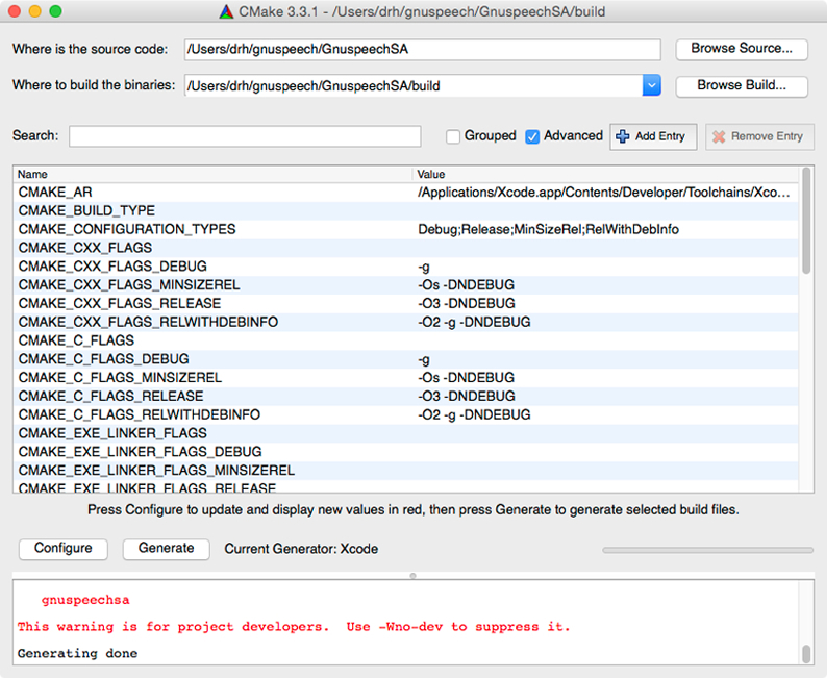
\includegraphics{images/cmake-window-after-generate}
\caption[CMake Build]{\label{sa-build}The ``CMake Window''---source \& build directories added}}
\end{figure}

The warning message concerning the MACOS\_PATH that appears (in red) can be ignored. A gnuspeech\_sa.xcode file will have been generated in the build directory. If not using using OS X 10.4 (``Yosemite") some parameter adjustment may be needed.

Double click the gnuspeech\_sa.xcode file to open Xcode and compile the sources. When the compilation is complete a ``Debug'' directory will be found in the build directory that contains a number of files, including the gnuspeech\_sa executable. If you change to the build directory and type the following command\footnote{\textbf{Note:} these two lines that follow actually represent a \emph{single} line with a space at the line-break instead of the new line.}:

\begin{verbatim}./gnuspeech\_sa -v -c ../../data/en -p trm_param_file.txt
-o do-you-happen.wav "Do you happen to know by chance what time it is?"
\end{verbatim}

\noindent{}followed by a Return. A .wav file of the spoken version of ``Do you happen to know by chance what time it is?'' will appear in the Debug folder after significant diagnostic output on the Terminal. To place the executable in its own directory, simply move or copy gnuspeech\_sa, along with the ``data'' directory and the trm\_param\_file.txt. Placement of the output file is determined by the ``-o'' parameter on the command line.

\href{https://youtu.be/NUrODiSkWk8}{\underline{{\textcolor{blue}{Here is an audio recording of the output}}}} generated by the command line above, when executed in the Debug directory.

\section
{Outline of Halliday's British English intonation notation}

\label{halliday}

\vspace{-6pt}
\begin{small}(The following summary is based on Halliday (1970). The book is out of print, but used copies are available in  many libraries and a few for sale---at Amazon, for example. Other relevant references to Halliday's work appear in the ``References'' section (Section \ref{refs}).
\end{small}

\subsection{British English Intonation}

Natural conversation in English involves continuous selection from five tones. Subdivisions depend on the ``delicacy'' used/required, which depends in turn on the requirements of the grammar. However, Halliday does not tie phonology directly to grammar---English is unfortunately (or more likely fortunately) not that simple. At the same time it is not enough to treat intonation systems as the emotional icing on the communication cake.

Intonation contrasts are \emph{not} lexical. Intonational and non-intonational aspects of grammar co-exist (Halliday 1967; 2004). Given that features of an intonation system may satisfy a variety of systems in the grammar, we should not fall into the trap of setting up a different intonation system for each role. This would add needless confusion. The concept of ``tone'' is an abstraction that provides a meaningful framework for the variations that occur in natural speech.

For purposes of characterising intonation, four types of unit are recognised:

\begin{itemize}
\item{the tone group, whose boundary is also a foot, syllable and phoneme boundary;}
\item{the foot---the basic rhythmic unit;}
\item{the syllable; and}
\item{the phoneme---closely related to the class of sounds produced by a particular posture.}
\end{itemize}

Following Abercrombie and Halliday, each foot begins with an accented syllable---the beat (see Allen 1972a; 1972b) and may be followed by weaker syllables. Halliday claims that some feet begin with a ``silent stress'' but, if so, this missing beat was seen to have zero duration in our analyses. Successive feet make up tone groups---of which there are five main categories, as noted, and in each simple tone group there is one obligatory foot for which the initial syllable---the ``tonic syllable''---receives ``tonic prominence'', making that foot the ``tonic foot''. The tonic represents the ``information'' point of the phrase, sentence or utterance. Feet occurring prior to the tonic, if any, make up the ``pretonic'' (which is optional), and feet after the tonic, if any, simply follow the tonic pitch movement at a reduced rate. The foot structure is determined by the occurrence of stressed syllables. In Gnuspeech, the dictionary includes an indication of which syllable in a given word can carry such stress (called ``word stress''). Generally words that can carry word stress are ``content words''---nounds, adjectives, \textellipsis{}, as opposed to the grammatical glue words known as ``form words'' (words such as ``and'', ``the'', ``of'', and ``to''). Syllables in form words and other unstressed syllables may be stressed for particular purposes (e.g. ``But what is \underline{the} reason you went.'', ``I said \underline{re}port, not \underline{de}port.'' This technique is overused in North American sports reporting---the terms ``\underline{off}ense'' and ``\underline{de}fense'' are good examples. The tonic may also be misplaced as when the ferry staff announce that ``This is an important safety an\underline{noun}cement.'' instead of ``This is an important \underline{safe}ty announcement.''

The tone groups are associated with the grammatical structure. They help to enhance the intelligibility of the utterances, partly through their rhythmic effect, and they also significantly affect their meaning at several levels---semantic and pragmatic.

The scheme for rhythm has usually been labelled as a ``theory of isochrony'', probably on the pre-instrumental perception that the beats occurred at more or less regular intervals. Objectively, the beats do \emph{not} occur at regular intervals. In fact the intervals may vary in length by a factor of 7:1 between the shortest and the longest. However, our work has shown clearly that---at least for the British English RP accent---the tonic and final feet do have durations in which the feet with more phones are somewhat shorter than would be expected from the natural (statistical) durations of the constituent phones (see Subsection \ref{int-rhythm}). Thus there is some justification for calling English---particularly British RP English---a ``stress-timed'' language in contrast to French, which is conventionally called a ``syllable-timed'' language, where syllables tend to be perceived as occurring at regular intervals. Listening to native speakers of these two language bears out this distinction, at least at the perceptual level.

In the tonic foot there is always pitch movement, and the greatest rate of change of pitch occurs on the tonic syllable. Halliday says that pretonic pitch is be ``level'' in some pretonics, but in practice there is some pitch movement all the time in all speech, so level is a relative term. The tonic and the pretonic are the only two places where a contrast between tone groups can be made.

Figure \ref{hal-sum} shows the five basic tone groups and their variants diagrammatically. There are also two compound tone groups---13 and 53---that are made up of two successive simple tone groups with no intervening pretonic; specifically  tone group 1 followed by a tone group 3; or tone group 5 followed by tone group 3. The second tone group in either case is the minor one. The major information is carried by the first tone group---tone group 1. The information in the second tone group (3 or 5) is subordinate to the information in the first, though related.

There are three distinct areas of choice in producing the intonation for an English utterance.

\begin{enumerate}
\item{``TONALITY'': the distribution into tone groups---number and location of the boundaries;}
\item{``TONICITY'': the choice of tonic syllables; and}
\item{``TONE'': the choice of primary and secondary tone patterns.}
\end{enumerate}

Natural tonality defaults to roughly one tone group per grammatical clause---the boundaries may not exactly coincide---and represents the distribution of information units.

Tonicity is constrained by the rhythm---the position of salient (stressed) syllables, and the speakers intention to convey the information point(s) of what is being uttered. Tonicity is clearly related to tonality. The neutral form places makes the first syllable of the last element of the grammatical structure, which corresponds to the first syllable of the last foot, the tonic syllable. A regular departure, deserving special mention is in ``wh-''  or information questions. The tonic them falls on the stressed syllable of the interrogative element(s).

An explanation of Tone, the different tones as illustrated in Figure \ref{hal-sum}, is necessarily more complex and can only be partial, asking ``what grammatical systems do these tones expound'', and presupposing an explicit grammar. The basic frame breaks tone into three moods, declarative, interrogative, and imperative, contrasted with ``moodless'' minor clauses [``neutral'' as opposed to marked??]. Tone 1 may be regarded as the neutral tone, for declarative statements, with variants for simple statements, listing statements, emphasis, and so on. Interrogatives are broken into polar---yes/no---and non-polar---``information'' questions. Yes/no questions involve a rising pitch in the tonic, but the tones involved are subject to subtle choice depending on the situation and informational context. Halliday gives a detailed exposition of when to use the various tone groups on the basis of categorising clauses/utterances into: statements; questions of the two kinds; commands; answers; and exclamations.

\begin{figure}[htb]
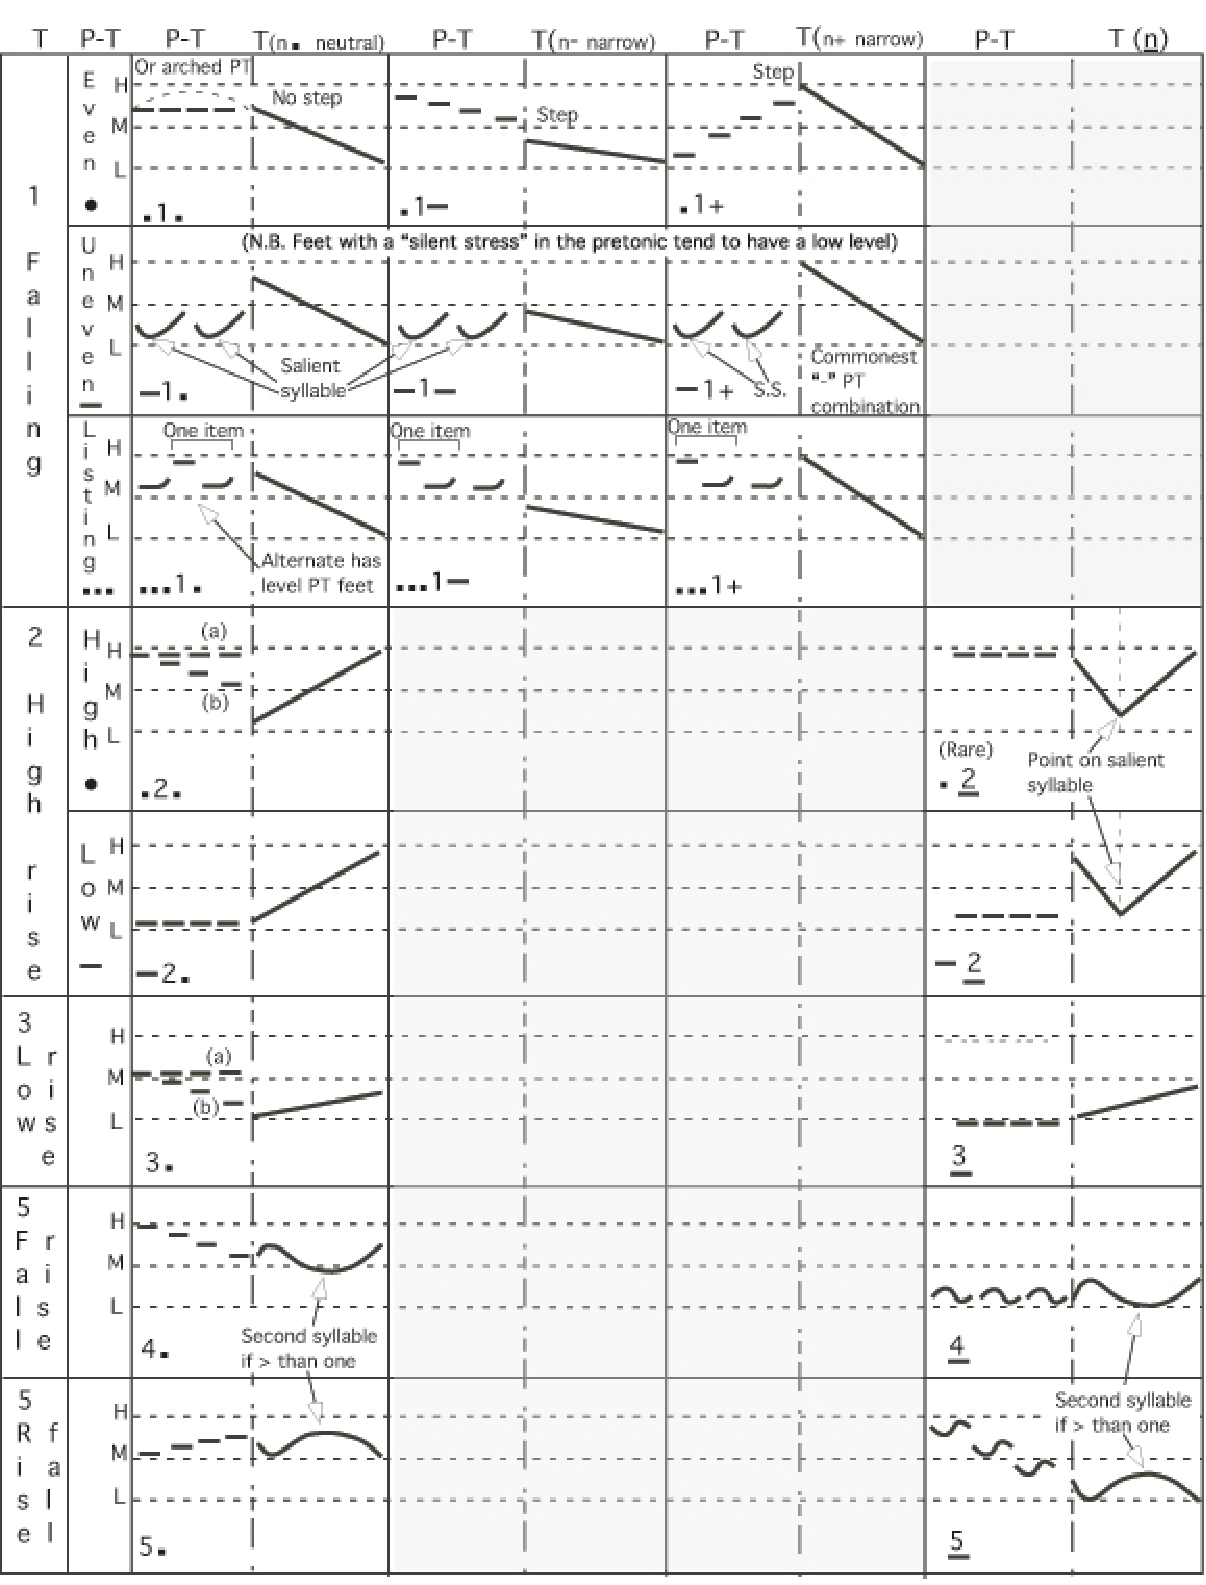
\includegraphics[width=16 cm]{images/halliday-summary}
\caption[Halliday tone-group summary]{A summary of the five tone groups and variants comprising the Halliday (1970) intonation system \label{hal-sum}}
\end{figure}

\clearpage

The reader is referred to Halliday's (1967) monograph for the full treatment, but this summary indicates the flavour. Even the full treatment is only a guide to the bones of British English intonation. Halliday says:
\begin{quotation}\begin{footnotesize}
Tone marks a kind of activity involved, by a complex pattern built out of simple opposition between certain and uncertain polarity. If the polarity is certain, the pitch of the tonic falls; if uncertain, it rises. Thus Tone 1 is an assertion, or a query not involving polarity; and Tone 4, which falls and then rises, is an assertion which involves or entails some query. Tone 2 is a query, \underline{2} being a query about a specific assertion; and tone 5, which rises and then falls, is a dismissed query, one countered by an assertion. Tone 2 avoids a decision; as an assertion it is at best confirmatory, contingent or immaterial.
\end{footnotesize}\end{quotation}

In his review of Halliday, Crystal criticises Halliday's thesis as based only on assertion, suggesting that Halliday has not shown that  intonation functions systemically in the same sense as grammar---see the Halliday (1967) citation. However, as a native speaker of RP English who has studied Halliday's work, and has been involved in the algorithmic synthesis and recognition of computer speech, it is clear to me that intonation and rhythm are essential components of meaning, and changes in intonation and rhythm dramatically affect both the basic meaning of utterances and the nuances that a speaker wishes to convey, not only by choice of words, but by choice of \emph{tonicity}, \emph{tonality} and \emph{tone}, as well as \emph{rhythm}. The problem remains concerning how to systematise the use of these feature of English. Halliday has made a giant step in that direction, but for high-quality synthesis and recognition by machine, algorithms to untangle and use both meaning and speaker's intent are crucial. Punctuation alone doesn't cut it.


\end{document}


